%Template pembuatan proposal skripsi.
\documentclass{jtetiskripsi}

%Untuk prefiks pada daftar gambar dan tabel
\usepackage[titles]{tocloft}
\renewcommand\cftfigpresnum{Gambar\  }
\renewcommand\cfttabpresnum{Tabel\   }

%Untuk hyperlink dan table of content
\usepackage{hyperref}

\newlength{\mylenf}
\settowidth{\mylenf}{\cftfigpresnum}
\setlength{\cftfignumwidth}{\dimexpr\mylenf+1.5em}
\setlength{\cfttabnumwidth}{\dimexpr\mylenf+1.5em}

%Untuk Bold Face pada Keterangan Gambar
\usepackage[labelfont=bf]{caption}

%-----------------------------------------------------------------
%Disini awal masukan untuk data proposal skripsi
%-----------------------------------------------------------------
\titleind{PENGEMBANGAN \emph{GATEWAY} BERBASIS \emph{EMBEDDED DEVICE} UNTUK INTEROPERABILITAS JARINGAN SENSOR NIRKABEL DAN PROTOKOL INTERNET}

\fullname{GUNTUR DHARMA PUTRA}

\idnum{09/284593/TK/35393}

\approvaldate{3 Februari 2014}

\degree{Sarjana Teknik Elektro}

\yearsubmit{2014}

\program{Teknik Elektro}

\dept{Teknik Elektro dan Teknologi Informasi}

\firstsupervisor{Sigit Basuki Wibowo, S.T., M.Eng.}
\firstnip{1976 0501 2002 12 1 002}

\secondsupervisor{Bimo Sunarfri Hantono, S.T., M.Eng.}
\secondnip{1977 0131 2002 12 1 003}

%-----------------------------------------------------------------
%Disini akhir masukan untuk data proposal skripsi
%-----------------------------------------------------------------

\begin{document}

\cover

\approvalpage

%-----------------------------------------------------------------
%Disini awal masukan Acknowledment
%-----------------------------------------------------------------
\acknowledgment
\begin{flushright}
\emph{Karya sederhana ini kupersembahkan \\
buat Bapak, Ibu,\\dan Adik tercinta}
\end{flushright}

%-----------------------------------------------------------------
%Disini awal masukan untuk Prakata
%-----------------------------------------------------------------
\preface
Segala puji dan syukur semata-mata hanya untuk Allah SWT, karena atas segala
rahmat, hidayah dan bantuan-Nya jualah maka akhirnya Tesis dengan judul
Analisis Teoretis Pemantulan dan Pembiasan Gelombang Elektromagnet Pada
Bahan Magnetik Non Linear Orde Dua ini telah selesai penulis susun.

Telah banyak bantuan yang penulis peroleh selama dalam penulisan Tesis ini
, untuk itu tak lupa penulis ucapkan terima kasih yang sebesar-besarnya
kepada:
\begin{enumerate}
\item{Bapak Sarjiya, S.T., M.T., Ph.D., selaku Ketua Jurusan Teknik Elektro dan Teknologi Informasi Fakultas Teknik Universitas Gadjah Mada.}
\item{Bapak...selaku dosen pembimbing pertama ...}
\item{Ibu... selaku dosen pembimbing kedua ...}
\item{Bapak... selaku dosen pembimbing akademis.}
\item{Bapak dan Mama yang selama ini telah sabar membimbing dan mendoakan
penulis tanpa kenal untuk selama-lamanya,}
\item{Prof. Drs. H. Muslim, Ph. D, selaku Pembimbing Utama, yang telah
memberikan ilmunya kepada penulis serta dengan penuh kesabaran membimbing penulis,}
\item{Drs. Kamsul Abraha, Ph. D, selaku Pembimbing Pendamping yang telah
memberikan inspirasi kepada penulis,} 
\item{Dr. Pekik Nurwantoro dan Dr. rer. nat. M. Farchani Rasyid
yang telah memperkenalkan sistem operasi LINUX dan \LaTeX{} kepada penulis serta
memberikan bimbingan penggunaan \LaTeX{} tersebut dengan sabar,} 
\item{Segenap staf dan karyawan di jurusan Fisika FMIPA UGM, yang telah
banyak bekerjasama dengan penulis selama belajar di FMIPA UGM,} 
\item{Sahabat saya M. Rizal Ginanjar, yang selalu bersedia membantu penulis ketika
menyelesaikan masalah-masalah komputer.} 
\end{enumerate}

Tesis ini tentunya tidak lepas dari segala kekurangan dan kelemahan, untuk itu
segala kritikan dan saran yang bersifat membangun guna kesempurnaan Tesis ini
sangat diharapkan. Semoga tesis ini dapat bermanfaat bagi kita semua dan lebih
khusus lagi bagi pengembagan ilmu fisika.

\begin{tabular}{p{7.5cm}c}
&Yogyakarta, 15 Januari 2014\\
&\\
&\\
&Penulis
\end{tabular}

%-----------------------------------------------------------------
%Disini akhir masukan untuk muka skripsi
%-----------------------------------------------------------------
\tableofcontents
\addcontentsline{toc}{chapter}{DAFTAR ISI}
\listoftables
\addcontentsline{toc}{chapter}{DAFTAR TABEL}
\listoffigures
\addcontentsline{toc}{chapter}{DAFTAR GAMBAR}

%-----------------------------------------------------------------
%Daftar Singkatan [Optional]
%-----------------------------------------------------------------
\singkatan
\noindent
\begin{tabular}{lp{3pt}l}

\textbf{A}\\
AP & & Access Point\\
\\

\textbf{F}\\
FTDI & & Future Technology Devices International\\
FUSE & & Filesystem in Userspace\\
\\

\textbf{J}\\
JTETI & & Jurusan Teknik Elektro dan Teknologi Informasi\\
\\

\textbf{L}\\
LAN & & Local Area Network\\
\\

\textbf{R}\\
RF & & Radio Frequency\\
\\

\textbf{S}\\
SFTP & & Secure Shell File Transfer Protocol\\
SSHFS & & Secure Shell Filesystem\\
\\

\textbf{U}\\
UGM & & Universitas Gadjah Mada\\
\\

\textbf{W}\\
WAP & & Wireless Access Point\\
WLAN & & Wireless Local Area Network\\
WSN & & Wireless Sensor Network\\

\end{tabular}

%-----------------------------------------------------------------
%Disini awal masukan Intisari
%-----------------------------------------------------------------
\begin{abstractind}
Penggunaan \emph{Wireless Sensor Network} (WSN) untuk gedung dan perumahan semakin populer karena dapat dimanfaatkan untuk berbagai kepentingan seperti \emph{home automation} dan \emph{home surveillance}. Oleh karena itu, untuk meningkatkan fleksibilitas penggunaan WSN, diperlukan sistem pengendalian yang dapat dikendalikan secara jarak jauh. Padahal pada umumnya, WSN dikendalikan oleh sebuah pengendali utama berada di sekitar tempat WSN itu berada.

Penelitian ini mengusulkan integrasi dari WSN dengan \emph{Internet Protocol} (IP) yang memungkinkan WSN dapat dikendalikan dimanapun dan dengan apapun asalkan masih terhubung dengan jaringan internet. Penelitian ini memanfaatkan infrastruktur jaringan data yang sangat populer dan terhubung ke internet, yaitu jaringan area lokal nirkabel atau dikenal dengan nama WiFi. Salah satu perangkat utama dalam jaringan WiFi adalah \emph{Access Point} (AP) yang berfungsi sebagai koordinator simpul. Selain itu, AP juga berfungsi sebagai gateway yang menghubungkan berbagai piranti yang terhubung padanya ke internet. Oleh karena itu, penelitian ini akan mengembangkan perangkat lunak yang akan ditanamkan ke dalam AP sehingga menjadikan AP mempunyai kemampuan sebagai gateway untuk kedua jaringan WiFi dan beberapa protokol WSN ke dalam jaringan internet.


\bigskip
\noindent
\textbf{Kata kunci :} \emph{wireless sensor network}, \emph{Internet Protocol}, WiFi, interoperabilitas.
\end{abstractind}

\begin{abstracteng}
\emph{
Wireless Sensor Network (WSN) usage for buildings and household has been increasingly popular because it offers many benefits, such as home automation and home surveilliance. Therefore, in order to increase WSN flexibility usage, remote controlling which enables administration is needed. In fact, generally WSN is controlled by a coordinator (sink node) which is located near the WSN area itself.}

\emph{
This research proposes integration of WSN and Internet Protocol (IP), that enables remote controlling and administration through the Internet Protocol stack. This research utilizes the wireless local area network or commonly known as WiFi. One of main components on this WiFi network is Access Point (AP) that acts as node coordinator. Furthermore, AP also serves as a gateway that connects multiple devices, that is connected to the AP, to the Internet. Therefore, this research will develop a software which is going to be implemented to the AP so that the AP has a capability as a gateway for both WiFi network and several WSN protocols to the Internet.}


\bigskip
\noindent
\textbf{\emph{Keywords :}} \emph{wireless sensor network, Internet Protokol, WiFi, interoperability}.
\end{abstracteng}
%-----------------------------------------------------------------
%Disini akhir masukan Intisari
%-----------------------------------------------------------------

%-----------------------------------------------------------------
%Disini awal masukan untuk Bab
%-----------------------------------------------------------------
%-------------------------------------------------------------------------------
% 								BAB I
% 							LATAR BELAKANG
%-------------------------------------------------------------------------------

\chapter{LATAR BELAKANG}

\section{Latar Belakang Masalah}
Lorem ipsum dolor sit amet, consectetuer adipiscing elit, sed diam nonummy nibh euismod tincidunt ut laoreet dolore magna aliquam erat volutpat. Ut wisi enim ad minim veniam, quis nostrud exerci tation ullamcorper suscipit lobortis nisl ut aliquip ex ea commodo consequat. Duis autem vel eum iriure dolor in hendrerit in vulputate velit esse molestie consequat, vel illum dolore eu feugiat nulla facilisis at vero eros et accumsan et iusto odio dignissim qui blandit praesent luptatum zzril delenit augue duis dolore te feugait nulla facilisi. Nam liber tempor cum soluta nobis eleifend option congue nihil imperdiet doming id quod mazim placerat facer possim assum.\cite{wibowo2013wireless,Raluca2008}.

\section{Rumusan Masalah}
Habeo perfecto in sea. Ea deleniti gloriatur pri, paulo mediocrem incorrupte sea ei. Ad mollis scripta per. Incorrupte sadipscing ne mel. Mel ex nonumy malorum epicurei. Ne per tota mollis suscipit. Ullum labitur vim ut, ea dicit eleifend dissentias sit. Duis praesent expetenda ne sed. Sit et labitur albucius elaboraret. Ceteros efficiantur mei ad. Hendrerit vulputate democritum est at, quem veniam ne has, mea te malis ignota volumus.


\section{Batasan Masalah}
Batasan masalah pada penelitian ini adalah:
\begin{enumerate}
\item Penelitian ini difokuskan pada interoperabilitas beberapa \emph{vendor} WSN dan protokol Internet.
\item Tipe WSN yang digunakan dalam penelitian ini dibatasi dua buah.
\item Pengujian yang dilakukan hanya sebatas eksperimen dalam lingkup laboratorium.
\item Purwarupa yang dihasilkan akan diimplementasikan pada sebuah \emph{Access Point} (AP).
\end{enumerate}


\section{Tujuan Penelitian}
Eros reprimique vim no. Alii legendos volutpat in sed, sit enim nemore labores no. No odio decore causae has. Vim te falli libris neglegentur, eam in tempor delectus dignissim, nam hinc dictas an.


\section{Manfaat Penelitian}
Pro omnium incorrupte ea. Elitr eirmod ei qui, ex partem causae disputationi nec. Amet dicant no vis, eum modo omnes quaeque ad, antiopam evertitur reprehendunt pro ut. Nulla inermis est ne. Choro insolens mel ne, eos labitur nusquam eu, nec deserunt reformidans ut. His etiam copiosae principes te, sit brute atqui definiebas id.

Et affert civibus has. Has ne facer accumsan argumentum, apeirian hendrerit persequeris pro ex. Suscipit vivendum sensibus mea at, vim ei hinc numquam, at dicit timeam dissentiet mel. At patrioque intellegebat sea, error argumentum dissentias sea in.


\section{Keaslian Penelitian}
No per amet modo comprehensam, duo dolor dignissim ex, ancillae corrumpit intellegam vix te. Mel utinam signiferumque no, ex nec accusam accumsan. Et per inermis posidonium, qui et ornatus epicuri pertinax. In homero commodo usu, vel te habemus fuisset, id nec periculis sententiae efficiendi. Oblique sanctus intellegat at cum.


\section{Sistematika Penulisan}
\noindent
\textbf{BAB I : PENDAHULUAN}

Pada bab ini dijelaskan latar belakang, rumusan masalah, batasan, tujuan, manfaat, keaslian penelitian, dan sistematika penulisan.\\

\noindent
\textbf{BAB II : TINJAUAN PUSTAKA DAN LANDASAN TEORI}

Pada bab ini dijelaskan teori-teori dan penelitian terdahulu yang digunakan sebagai acuan dan dasar dalam penelitian.\\

\noindent
\textbf{BAB III : METODOLOGI PENELITIAN}

Pada bab ini dijelaskan metode yang digunakan dalam penelitian meliputi langkah kerja, pertanyaan penilitian, alat dan bahan, serta tahapan dan alur penelitian.\\

\noindent
\textbf{BAB IV : HASIL DAN PEMBAHASAN}

Pada bab ini dijelaskan hasil penelitian dan pembahasannya.\\

\noindent
\textbf{BAB V : KESIMPULAN DAN SARAN}

Pada bab ini ditulis kesimpulan akhir dari penelitian dan saran untuk pengembangan penelitian selanjutnya.\\

% Baris ini digunakan untuk membantu dalam melakukan sitasi
% Karena diapit dengan comment, maka baris ini akan diabaikan
% oleh compiler LaTeX.
\begin{comment}
\bibliography{daftar-pustaka}
\end{comment}


%-------------------------------------------------------------------------------
%                            BAB II
%               TINJAUAN PUSTAKA DAN DASAR TEORI
%-------------------------------------------------------------------------------

\chapter{TINJAUAN PUSTAKA DAN DASAR TEORI}                

\section{Tinjauan Pustaka}
  Secara umum, cara untuk menghubungkan WSN dengan jaringan internet dapat dikelompokkan menjadi dua. Cara pertama adalah menggunakan gateway dan cara yang kedua adalah dengan menggunakan simpul sensor yang sudah dilengkapi dengan protokol internet. Cara yang lebih mudah ditempuh adalah dengan cara yang pertama karena pengubahan yang dilakukan relatif tidak terlalu besar. Sedangkan cara yang kedua akan menemui banyak kendala terutama pada WSN yang sudah terpasang karena harus dilakukan penggantian tiap simpul sensor.

  Salah satu usaha untuk mengintegrasikan jaringan WSN dengan jaringan WiFi menggunakan gateway misalnya dilakukan pada penelitian. Pada riset tersebut pengintegrasian dilakukan dengan sebuah komputer yang didedikasikan untuk keperluan tertentu. Penggunaan komputer khusus ini adalah hardware-solution yang membutuhkan biaya dan kerumitan sistem.

  Riset pada juga menawarkan pengintegrasian dengan jaringan IP. Namun demikian di dalam riset ini diperlukan perubahan yang signifikan jika konfigurasi jaringan sensor nirkabel sudah terpasang. Simpul sensor yang digunakan harus diganti dengan simpul sensor yang mendukung IP. Hal ini jelas akan memakan biaya yang cukup besar dan tidak praktis untuk dilakukan. Terlebih lagi jika jumlah sensor yang terpasang jumlahnya cukup banyak.

  Riset pada sudah berhasil mengembangkan sebuah AP menjadi gateway yang dapat digunakan untuk menghubungkan sebuah protokol WSN dengan jaringan IP. Protokol WSN yang digunakan adalah protokol dari IQRF. Penelitian tersebut kemudian dilanjutkan dengan penelitian yang sudah diterapkan dalam sistem domotic.

\section{Landasan Teori}
  \subsection{\emph{Wireless Sensor Network}}
    Jaringan sensor nirkabel (Wireless Sensor Network, WSN) adalah jaringan simpul sensor otonom yang terdistribusi digunakan untuk memonitor kondisi fisik atau lingkungan misalnya suhu, suara, getaran, kelembaban, dan lain-lain. Selain itu, tidak menutup kemungkinan untuk menambahkan fungsi tambahan pada setiap simpul misalnya port masukan/keluaran (I/O port) yang terdapat dalam setiap simpul dihubungkan dengan aktuator sehingga dapat digunakan untuk mengendalikan piranti elektrik atau elektronis.

    Secara umum, WSN dapat diilustrasikan seperti Gambar \ref{wsn}. Pada gambar tersebut terlihat adanya beberapa simpul yang diwakili dengan titik berukuran kecil dan satu buah simpul yang diwakili dengan titik berukuran lebih besar. Titik yang berukuran kecil mewakili simpul sensor sedangkan titik yang berukuran besar mewakili gateway yang berfungsi menghubungkan jaringan sensor nirkabel dengan pengendali utama yang dalam gambar tersebut diwakili oleh sebuah komputer. Contoh sebuah simpul dari IQRF ditunjukkan pada Gambar \ref{iqrf}.

      \begin{figure}[ht!]
        \centering
          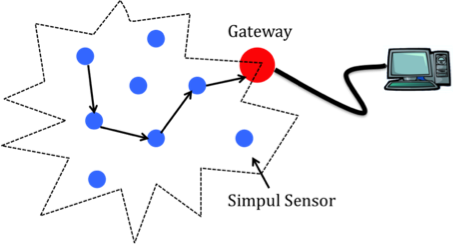
\includegraphics{gambar/wsn}
          \caption{Jaringan sensor nirkabel.}
          \label{wsn}
      \end{figure}

    Pada umumnya, WSN adalah jaringan yang berdiri sendiri. Untuk menghubungkan WSN dengan jaringan yang lain misalnya jaringan internet, maka salah satu cara adalah dengan membangun gateway WSN yang mampu menjembatani perbedaan protokol yang ada pada WSN dan jaringan internet. Cara tersebut adalah cara yang ditempuh dalam penelitian ini karena lebih mudah dilakukan dibandingkan dengan cara yang lain seperti sudah dijelaskan pada Bab Tinjauan Pustaka.

      \begin{figure}[ht!]
        \centering
          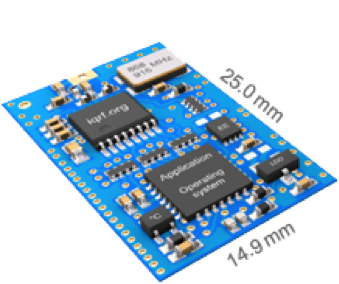
\includegraphics{gambar/iqrf}
          \caption{Contoh sebuah simpul sensor IQRF.}
          \label{iqrf}
      \end{figure}

    Sementara itu, jaringan WiFi sebagai jaringan lokal nirkabel yang digunakan untuk komunikasi data dalam suatu area lokal dan sudah tersebar di berbagai tempat. Lokal yang dimaksud disini adalah area yang tidak terlalu luas yaitu dengan radius sekitar 20m atau dalam sebuah gedung. Untuk membangun jaringan lokal menggunakan WiFi, perangkat utama yang digunakan adalah Access Point (AP). AP adalah piranti yang akan menjadi koordinator dalam jaringan lokal jika diinginkan topologi bintang (star) seperti diilustrasikan pada Gambar \ref{star}.

      \begin{figure}[ht!]
        \centering
          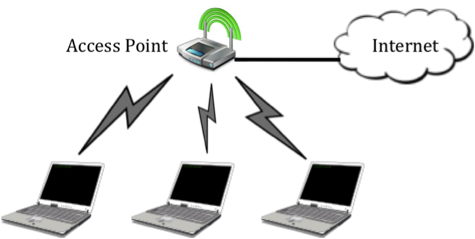
\includegraphics{gambar/star}
          \caption{Jaringan bintang menggunakan WiFi.}
          \label{star}
      \end{figure}

    Gambar \ref{star} memberi ilustrasi sebuah jaringan WiFi yang terdiri dari tiga buah komputer dan satu buah AP yang terhubung ke jaringan internet. Dengan konfigurasi tersebut, semua komputer yang ada di dalam jaringan WiFi dapat berkomunikasi dengan internet dengan aturan yang ditentukan oleh AP.

    Jika dilihat lebih dalam lagi, AP ini sebenarnya adalah piranti tertanam (embedded device) yang didalamnya sudah terdapat pusat pengolahan utama, memory, dan penyimpanan (storage). Dengan kenyataan inilah maka AP mempunyai potensi untuk menjagi gateway bagi jaringan WiFi dan WSN ke jaringan internet. Untuk mengembangkan aplikasi yang akan ditanamkan ke dalam AP, maka diperlukan sistem operasi yang sesuai untuk AP.

  \subsection{IQRF}
    IQRF adalah teknologi komunikasi nirkabel berbasis paket melalui frekuensi radio dalam pita frekuensi sub-GHz. Teknologi ini dimaksudkan untuk penggunaan umum saat konektivitas nirkabel dibutuhkan, entah \emph{point to point} atau jaringan yang kompleks. fungsionalitas lengkapnya bergantung semata-mata pada aplikasi berbahasa C yang ditulis oleh pengguna.

    Peranti kominikasi dasar dari IQRF adalah sebuah modul pancar-rima termasuk unit mikrokontroler dengan sistem operasi tertanam yang mengimplementasikan lapisan \emph{link} dan lapisan jaringan yang mendukung jaringan jala (\emph{mesh}) dengan protokol IQMESH. Tidak ada tingkat komunikasi yang lebih tinggi seperti lapisan \emph{transport} yang termasuk kedalam teknologi ini.

    Fitur-fitur yang dimiliki antara lain:
      \begin{itemize}
        \item Kecepatan, daya, dan ukuran data yang rendah,
        \item RF yang berbasis paket data, maksimal 128 Byte per paket,
        \item pita frekuensi sub-GHz (868 MHz, 916 MHz, dst.), \emph{multichannel}, dan modulasi FSK,
        \item \emph{bit rate} 1.2 kb/s – 86.2 kb/s,
        \item daya keluaran maksimal 20 mW,
        \item maksimal 65.000 peranti dalam satu jaringan,
        \item konsumsi daya yang rendah: 380 nA saat \emph{standby}, 25 µA saat menerima.
      \end{itemize}


  \subsection{XBee}
    XBee adalah sebuah merk dari Digi International untuk keluarga modul radio. XBee pertama diperkenalkan dalam merk MaxStream pada tahun 2005 yang berdasarkan pada standar IEEE 802.15.4-2003 untuk \emph{point to point} dan komunikasi bintang dalam \emph{baud rate} 250 kbit/s.

      \begin{figure}[ht!]
        \centering
          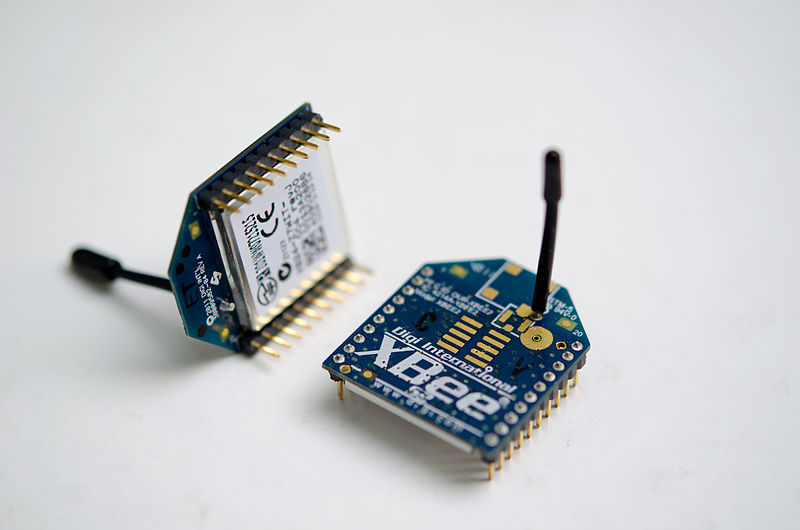
\includegraphics[width=0.5\textwidth]{gambar/xbee}
          \caption{Sepasang peranti XBee.}
          \label{xbee}
      \end{figure}

    Pada awalnya diperkenalkan dua model, yaitu 1mW XBee dan 100mW XBee-PRO. Sejak pertama kali diperkenalkan, beberapa buah XBee baru juga diperkenalkan dan semua XBee sekarang dipasarkan dengan merk Digi. Contoh peranti XBee dapat dilihat pada Gambar \ref{xbee}.

  \subsection{TCP/IP}
    Protokol internet adalah kumpulan protokol-protokol komunikasi yang digunakan dalam internet dan jaringan komputer sejenis, dan umumnya merupakan protokol yang paling populer untuk WAN. Pada umumnya hal ini dikenal dengan TCP/IP, karena protokol utamanya merupakan protokol jaringan pertama yang terstandarisasi. Terkadang hal ini dikenal dengan model DoD karena pengaruh ARPANET pada dekade 1970an.

    TCP/IP menyediakan konektivitas antar ujung yang menspesifikasikan bagaimana data harus diformat, dialamatkan, ditransmisikan, dirutekan, dan diterima di tujuan. TCP/IP memiliki empat layer abstraksi yang digunakan untuk mengurutkan semua protokol internet menurut jangkauan jaringan yang terlibat. Dari terendah sampai tertinggi, lapisan-lapisan tersebut adalah layer link, layer internet, layer transport, dan layer aplikasi.

  \subsection{\emph{Access Point}}
    \emph{Access Point}, disingkat AP, atau juga dikenal dengan istilah \emph{Wireless Access Point} adalah sebuah peranti yang memungkinkan peranti-peranti nirkabel untuk terkoneksi dengan jaringan kabel menggunakan Wi-Fi atau standar lain. AP biasanya terkoneksi dengan sebuah \emph{router} (melalui jaringan kabel) sebagai peranti yang berdiri sendiri, namun juga dapat menjadi bagian dalam komponen \emph{router} tersebut.

    Penggunaan secara korporat melibatkan beberapa AP ke dalam jaringan kabel dan menyediakan akses nirkabel ke LAN kantor. AP diatur dengan WLAN \emph{Controller} yang menangani pengaturan daya RF, kanal-kanal, autentikasi, dan keamanan.
    
    Sebuah \emph{hotspot} adalah aplikasi dari satu atau beberapa AP, di mana peranti dapat terhubung ke Internet dengan mudah. Konsep ini sudah menjadi hal yang umum di beberapa kota besar, di mana kombinasi dari warung kopi, perpustakaan, dan AP milik pribadi memungkinkan klien untuk terkoneksi dengan Internet. Koleksi dari \emph{hotspot} yang terkoneksi dapat disebut sebagai sebuah jaringan \emph{lili pad}.

  \subsection{Web Server}
    Web server dapat mengacu pada perangkat keras atau perangkat lunak yang membantu dalam penyampaian konten web yang dapat diakses melalui internet.

    Penggunaan web server yang paling umum adalah sebagai host untuk halaman web, walaupun ada beberapa penggunaan lain seperti game, media penyimpan data, atau penjalanan aplikasi perusahaan.


  \subsection{AJAX}
    AJAX adalah kelompok dari teknik-teknik pengembangan web yang digunakan pada klien untuk membuat aplikasi asinkron. Dengan AJAX, aplikasi web dapat mengirim dan menerima data dari sebuah server secara asinkron tanpa mengganggu tampilan dari halaman yang ada. Data dapat diambil menggunakan obyek XMLHttpRequest. Penggunaan XML tidak diperlukan, malahan JSON lebih sering digunakan, dan rekues tidak harus asinkron.

    AJAX bukanlah sebuah teknologi, tapi kelompok dari teknologi-teknologi. HTML dan CSS dapat digunakan dalam kombinasi untuk mark up dan informasi tampilan. DOM diakses oleh JavaScript untuk menampilkan dan mengijinkan pengguna untuk berinteraksi dengan informasi tertampil. JavaScript dan obyek XMLHttpRequest menyediakan sebuah metode untuk pertukaran data secara asinkron antara browser dan server untuk menghindari muat ulang halaman secara keseluruhan.


  \subsection{OpenWRT}
    OpenWRT adalah sebuah sistem operasi untuk \emph{embedded device} yang berbasis pada Linux kernel. OpenWRT pada umumnya digunakan dalam routing \emph{network traffic}. Komponen-komponen utamanya adalah Linux kernel, util-linux, uClibc dan BusyBox. Semua komponen sudah dioptimalkan dan dimampatkan untuk bisa muat dalam \emph{router} rumahan yang memiliki keterbatasan media penyimpan dan memori. OpenWRT dapat dikonfigurasikan melalui antarmuka \emph{command-line} (\emph{ash shell}), seperti dapat dilihat pada Gambar \ref{openwrt}, atau dengan antarmuka Web (LuCI). Terdapat kurang lebih 3.500 paket-paket perangkat lunak tambahan yang tersedia untuk diinstal melalui sistem manajemen paket \emph{opkg}.

      \begin{figure}[ht!]
        \centering
          
\includegraphics[width=10cm]{gambar/openwrt}
          \caption{Tampilan antarmuka \emph{command-line} OpenWRT versi \emph{BackFire}.}
          \label{openwrt}
      \end{figure}

    OpenWRT dapat berjalan pada router CPE (\emph{Customer Premised Equipment}), \emph{gateway} residensial, komputer saku (seperti Ben NanoNote), dan komputer jinjing. OpenWRT juga dapat berjalan pada komputer konvensional atau komputer dengan arsitektur x86. Banyak \emph{patch} dari kode sesumber berbasis OpenWRT yang diubah kedalam Linux kernel utama.

  \subsection{SSHFS}
    SSHFS (SSH Filesystem) adalah sebuah klien \emph{filesystem} untuk \emph{mount} dan berinteraksi dengan direktori dan arsip yang berlokasi pada server atau \emph{workstation}. Klien berinteraksi dengan server dengan SSH \emph{File Transfer Protocol} (SFTP), sebuah protokol jaringan yang menyediakan akses ke arsip, transfer arsip, dan fungsionalitas manajemen arsip melalui aliran data yang didesain sebagai ekstensi dari protokol SSH versi 2.0.

  \subsection{Bootstrap}
    Bootstrap adalah koleksi gratis dari alat-alat untuk membuat situs web dan aplikasi berbasis web. Bootstrap terdiri dari HTML dan contoh desain berbasis CSS untuk tipografi, borang, tombol, navigasi, komponen antarmuka lain, dan juga ekstensi JavaScript yang bersifat opsional.

    Bootstrap merupakan proyek paling populer pada GitHub, dan sudah digunakan oleh, diantaranya, NASA dan MSNBC.


%-------------------------------------------------------------------------------
%                            BAB III
%               		METODOLOGI PENELITIAN
%-------------------------------------------------------------------------------

\chapter{METODOLOGI PENELITIAN}

\section{Alat dan Bahan}
	Alat dan bahan yang digunakan pada penelitian ini terbagi atas perangkat keras dan perangkat lunak yang akan dijelaskan seperti berikut.

	\subsection{Perangkat Keras}
		Pro omnium incorrupte ea. Elitr eirmod ei qui, ex partem causae disputationi nec. Amet dicant no vis, eum modo omnes quaeque ad, antiopam evertitur reprehendunt pro ut. Nulla inermis est ne. Choro insolens mel ne, eos labitur nusquam eu, nec deserunt reformidans ut. His etiam copiosae principes te, sit brute atqui definiebas id.

		\vspace{-0.5cm}

		\begin{enumerate}[a.]
		\begin{singlespace}
		\itemsep0em
			\item Kit pancar-rima IQRF TR-53B (3 unit),
			\item Kit pengunduh program CK-USB-04 (1 unit),
			\item Kit pengembangan DK-EVAL-03 (2 unit),
			\item Kit pengembangan CK-EVAL-04 (1 unit),
			\item \emph{XBee 802.15.4 Radios (Series 1)} (3 unit),
			\item \emph{XBee Explorer USB Board} (1 unit),
			\item \emph{2 channel Relay Shield For Arduino (With XBee/BTBee interface)} (2 unit),
			\item Arduino Uno (2 unit),
			\item TP-LINK MR3020 (1 unit),
			\item Kabel USB ke Serial Prolific (1 unit).
		\end{singlespace}
		\end{enumerate}

	\subsection{Perangkat Lunak}
		Pro omnium incorrupte ea. Elitr eirmod ei qui, ex partem causae disputationi nec. Amet dicant no vis, eum modo omnes quaeque ad, antiopam evertitur reprehendunt pro ut. Nulla inermis est ne. Choro insolens mel ne, eos labitur nusquam eu, nec deserunt reformidans ut. His etiam copiosae principes te, sit brute atqui definiebas id.

		\vspace{-0.5cm}

		\begin{enumerate}[a.]
		\begin{singlespace}
		\itemsep0em
			\item Arduino for Mac OS X,
			\item CoolTerm,
			\item Driver FTDI for Mac OS X,
			\item PHP, MySQL, dan uHTTPd,
			\item Python dan pustaka PySerial,
			\item IQRF IDE v 2.08 for TR-53B,
			\item SSHFS,
			\item Sublime Text 3.
		\end{singlespace}
		\end{enumerate}

\section{Alur Penelitian}
	Consul graeco signiferumque qui id, usu eu summo dicunt voluptatum, nec ne simul perpetua posidonium. Eos ea saepe prodesset signiferumque. No dolore possit est. Mei no justo intellegebat definitiones, vis ferri lorem eripuit ad. Solum tritani scribentur duo ei, his an adipisci intellegat.

\section{Tahapan Pelaksanaan}
	Consul graeco signiferumque qui id, usu eu summo dicunt voluptatum, nec ne simul perpetua posidonium. Eos ea saepe prodesset signiferumque. No dolore possit est. Mei no justo intellegebat definitiones, vis ferri lorem eripuit ad. Solum tritani scribentur duo ei, his an adipisci intellegat.

\section{Jadwal Kegiatan}
	Quo no atqui omnesque intellegat, ne nominavi argumentum quo. Eum ei purto oporteat dissentiet, soleat utamur an sit. Et assum dicam interpretaris quo. Cetero alterum ea vel, no possit alterum utroque nec. His fuisset quaestio ad. Has eu tritani incorrupte consequuntur, esse aliquip nec ne \ref{jadwal}.

	% Please remember to add \use{multirow} to your document preamble in order to suppor multirow cells
		\begin{table}[H]
		\centering
		\caption{Jadwal Penelitian.}
		\label{jadwal}
		\begin{tabular}{|c|l|l|l|l|l|l|l|}
		\hline
		\multirow{2}{*}{No} & \multirow{2}{*}{Keterangan} & \multicolumn{6}{c|}{Bulan}                                                                                                                          \\ \cline{3-8} 
		                    &                             & 1 & 2 & 3 & 4 & 5 & 6 \\ \hline
		1                   & Studi literatur                                  &\cellcolor{gray} &\cellcolor{gray}&                        &                        &                        &                         \\ \hline
		2                   & Desain                                           &                        &\cellcolor{gray}&\cellcolor{gray}&                        &                        &                         \\ \hline
		3                   & Pembelian bahan                                  &                        &                        &\cellcolor{gray}&                        &                        &                         \\ \hline
		4                   & Pembuatan prototipe                              &                        &                        &\cellcolor{gray}&\cellcolor{gray}&\cellcolor{gray}&                         \\ \hline
		5                   & Uji coba dan perbaikan                           &                        &                        &                        &\cellcolor{gray}&\cellcolor{gray}&                         \\ \hline
		6                   & Penulisan skripsi                                &                        &                        &                        &                        &                        &\cellcolor{gray}\\ \hline
		\end{tabular}
		\end{table}
	
% Baris ini digunakan untuk membantu dalam melakukan sitasi
% Karena diapit dengan comment, maka baris ini akan diabaikan
% oleh compiler LaTeX.
\begin{comment}
\bibliography{daftar-pustaka}
\end{comment}


%-------------------------------------------------------------------------------
%                            BAB IV
%               		HASIL DAN PEMBAHASAN
%-------------------------------------------------------------------------------

\chapter{HASIL DAN PEMBAHASAN}
	\section{Analisis Kebutuhan Sistem}
		Bagian ini menjelaskan hal-hal yang terkait tentang pengembangan aplikasi sebelum penulisan code sesumber.

		\subsection{Fitur-Fitur Aplikasi}
			Kemampuan utama dari aplikasi yang dibangun adalah dapat mengendalikan sensor-sensor yang terhubung dengan \emph{gateway}. Pengendalian yang dimaksud adalah menyala-matikan \emph{relay} dan membaca temperatur yang terbaca. Selain itu, aplikasi juga dapat menambahkan sensor baru atau menghapus sensor lama. Untuk mendukung automatisasi, aplikasi juga dapat menjalankan \emph{profile} tertentu dari kombinasi suhu dan relay atau waktu tertentu. Kemampuan aplikasi dapat dilihat pada daftar berikut.

			\vspace{-0.5cm}

			\begin{itemize}
			\begin{singlespace}
				\item Mampu membaca dan menampilkan suhu yang terbaca pada sensor IQRF,
				\item mampu menyala-matikan relay pada peranti yang diinginkan,
				\item mampu menambah dan mengurangi peranti baru baik IQRF atau XBee,
				\item mampu menjalankan \emph{profile} tertentu dari kombinasi suhu dan relay atau waktu tertentu.
			\end{singlespace}
			\end{itemize}

			Pengguna diharuskan untuk \emph{login} terlebih dahulu sebelum dapat menggunakan aplikasi. Jika pengguna terdaftar sebagai \emph{administrator} maka pengguna tersebut dapat menambahkan pengguna baru, menghapus akun pengguna, mengangkat dan menurunkan pengguna menjadi \emph{administrator}. Kemampuan aplikasi dalam menangani pengguna dapat dilihat pada daftar berikut.

			\vspace{-0.5cm}
			\begin{itemize}
			\begin{singlespace}
				\item Mengharuskan pengguna untuk memasukkan nama dan kata sandi sebelum masuk ke aplikasi,
				\item dapat menambah atau mengurangi pengguna yang dapat memasuki sistem.
			\end{singlespace}
			\end{itemize}

		\subsection{\emph{Use Case Diagram}}
			Aktor yang terlibat dalam aplikasi ini hanya satu seperti yang tertera pada Gambar \ref{usecase}. Untuk memanfaatkan semua fitur yang ada pada aplikasi, pengguna diharuskan untuk \emph{login} terlebih dahulu. \emph{Case-case} yang ada pada aplikasi ini adalah, membaca suhu, menambah-kurangi sensor IQRF, menambah-kurangi sensor XBee, menyala-matikan relay, dan menambah-kurangi pengguna baru, seperti yang tergambar pada Gambar \ref{usecase}.

				\begin{figure}[H]
				  \centering
				    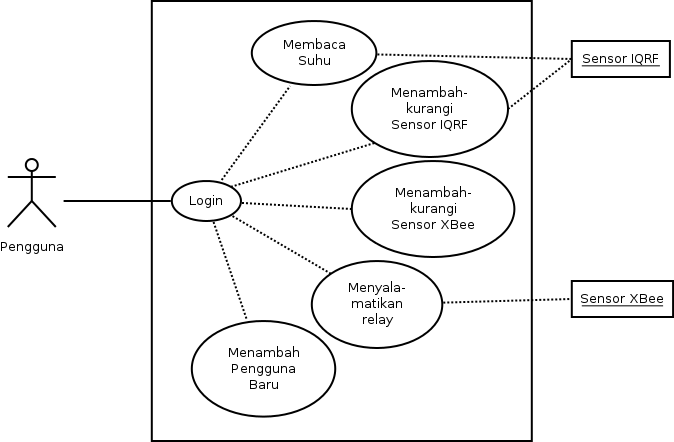
\includegraphics[width=0.9\textwidth]{gambar/usecase}
				    \caption{Diagram \emph{use case} dari penelitian.}
				    \label{usecase}
				\end{figure}

			Pada Gambar \ref{usecase}, menambah-kurangi sensor XBee tidak melibatkan sensor XBee (tidak ada garis yang menghubungkan keduanya), pada \emph{case} tersebut hanya melibatkan aplikasi. Saat \emph{case} ini dijalankan, data sensor pada basis data dihapus. Namun, menambah-kurangi sensor IQRF melibatkan sensor IQRF (ada garis yang menghubungkan keduanya). Karena pada \emph{case} ini, selain menghapus data pada basis data, proses \emph{unbonding} pada IQRF juga melibatkan \emph{node} IQRF.

		\subsection{Diagram Arsitektur Sistem}
			Penelitian ini menggunakan AP, \emph{sensor coordinator}, dan \emph{sensor node} sebagai peranti keras. Sedangkan peranti lunak yang dikembangkan meliputi aplikasi berbasis web, aplikasi Python, dan aplikasi C yang terunggah pada sensor-sensor. Gambar \ref{system-architecture} menggambarkan diagram arsitektur sistem.
			
			\begin{figure}[H]
			  \centering
			    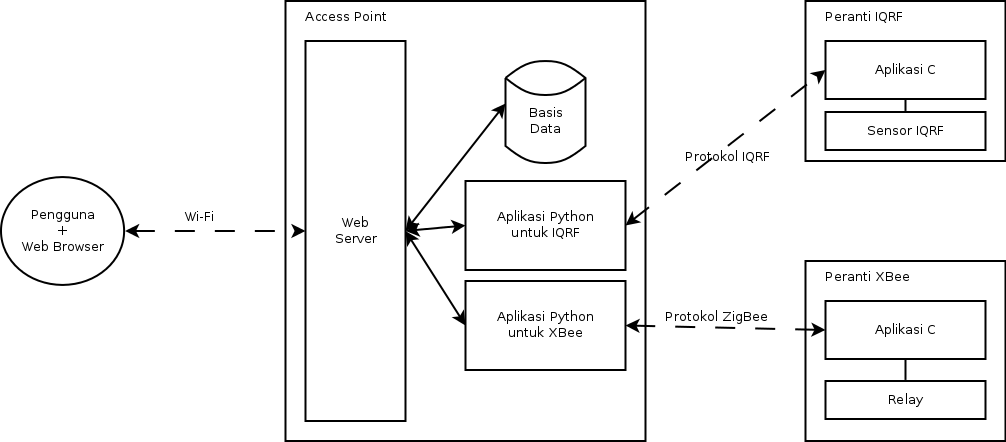
\includegraphics[width=\textwidth]{gambar/system-architecture}
			    \caption{Diagram Arsitektur Sistem.}
			    \label{system-architecture}
			\end{figure}

			Seperti terlihat pada Gambar \ref{system-architecture}, pengguna yang ingin mengakses aplikasi berbasis web guna mengendalikan sensor harus menggunakan web browser. Web browser yang dimaksud tidak terbatas hanya yang terinstal pada komputer, namun juga web browser yang terdapat pada ponsel cerdas atau komputer tablet.

		\subsection{SDLC}
			SDLC yang digunakan dapat dilihat pada Gambar \ref{sdlc}.
			\begin{figure}[H]
			  \centering
			    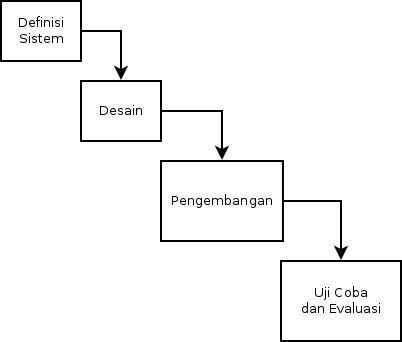
\includegraphics[width=0.6\textwidth]{gambar/sdlc}
			    \caption{Diagram SDLC.}
			    \label{sdlc}
			\end{figure}
	
	\section{Pengembangan Aplikasi}
		Tahap-tahap dalam pengembangan aplikasi adalah persiapan, pengembangan aplikasi WSN yang ditulis dengan bahasa C, pengembangan aplikasi Python untuk menghubungkan aplikasi web dan sensor, pengembangan aplikasi berbasis web, serta evaluasi dan perbaikan.

		\subsection{Persiapan Pra Pengembangan Aplikasi}
			Persiapan yang harus dilakukan sebelum mengembangkan aplikasi adalah mengkonfigurasi router/AP, mengkonfigurasi komputer yang akan digunakan untuk pengembangan aplikasi, dan mengkonfigurasi pengalamatan pada XBee.

			\begin{enumerate}
				\item Konfigurasi Router/AP

					Penelitian ini menggunakan AP keluaran TP-LINK seri MR3020. AP jenis ini dipilih karena bentuknya yang kecil sehingga mudah dibawa atau dipindahkan dan kemudahannya untuk dimodifikasi. TP-LINK MR3020 juga terbilang populer di ranah komunitas sistem benam (\emph{embedded device}) sehingga memiliki dukungan yang baik dari pabrikan dan komunitas. 

					Sebelum digunakan, \emph{firmware} bawaan TP-LINK MR3020 harus diganti dengan sistem operasi OpenWRT. Proses penggantian cukup mudah karena hanya memanfaatkan menu \emph{firmware upgrade} dari web admin yang sudah tersedia.	Sistem Operasi OpenWRT yang digunakan adalah Attitude Adjustment versi 12.09 dengan Linux kernel 3.3.8. \emph{Image file} sistem operasi tersebut bisa diunduh secara gratis pada situs \url{www.openwrt.org}.

					Setelah OpenWRT berhasil terinstall, langkah selanjutnya adalah mengimplementasikan \emph{extroot}. \emph{Extroot} dapat memperbesar memori penyimpanan dengan bantuan USB \emph{flash drive}. Langkah yang harus dilakukan pertamakali adalah menginstall perangkat lunak dengan perintah sebagai berikut:
					\begingroup
					    \fontsize{10pt}{12pt}\selectfont
					    \begin{verbatim}
							# opkg update
							# opkg install block-extroot block-hotplug block-mount
					    \end{verbatim}  
					\endgroup

					Kemudian dilanjutkan dengan menyalin isi dari memori internal TP-LINK MR3020 ke USB \emph{flash drive} yang di-\emph{mount} pada direktori /mnt/sda1 dengan perintah:
					\begingroup
					    \fontsize{10pt}{12pt}\selectfont
					    \begin{verbatim}
							# tar -C /overlay -cvf - . | tar -C /mnt/sda1 -xf -
					    \end{verbatim}  
					\endgroup

					Langkah terakhir adalah mengkonfigurasi file /etc/config/fstab dan menyalakan ulang AP. Konfigurasi diganti dengan detil sebagai berikut:
					\begingroup
					    \fontsize{10pt}{12pt}\selectfont
					    \begin{verbatim}
							config mount
						        option target        /mnt
						        option device        /dev/sda1
						        option fstype        ext3
						        option options       rw,sync
						        option enabled       1
						        option enabled_fsck  0
						        option is_rootfs     1
					    \end{verbatim}  
					\endgroup

					Setelah proses implementasi extroot selesai, berarti AP sudah memiliki memori penyimpanan yang cukup (atau mungkin lebih) untuk menginstal aplikasi-aplikasi pendukung lainnya. Penelitian ini menggunakan memori USB 4 Gigabyte.

					Agar TP-LINK MR3020 dapat membaca dan mengirimkan data dari dan ke WSN melalui kanal serial, dibutuhkan Python dan pustaka PySerial yang diinstal dengan perintah:
					\begingroup
					    \fontsize{10pt}{12pt}\selectfont
					    \begin{verbatim}
							# opkg update
							# opkg install python pyserial
					    \end{verbatim}  
					\endgroup

					Sedangkan paket aplikasi `at' digunakan agar AP dapat menjalankan perintah untuk menyala-matikan relay pada waktu tertentu. Namun, sebelum at dapat berjalan, pada router sudah harus tersedia file /var/spool/cron/atjobs/.SEQ dan pemilik dari file tersebut harus diganti menjadi daemon.daemon. Aplikasi `at' diinstall dengan perintah:
					\begingroup
					    \fontsize{10pt}{12pt}\selectfont
					    \begin{verbatim}
							# opkg update && opkg install at
					    \end{verbatim}  
					\endgroup
					
					Langkah selanjutnya adalah instalasi aplikasi pendukung aplikasi berbasis web yang nantinya akan dikembangkan yaitu Web Server, PHP, dan MySQL. Web server yang digunakan adalah yang sudah terinstal pada OpenWRT versi Attitude Adjustment yaitu uHTTPd. Sedangkan PHP dan MySQL harus diinstal dengan perintah:
					\begingroup
					    \fontsize{10pt}{12pt}\selectfont
					    \begin{verbatim}
							# opkg update
							# opkg install php5 php5-cgi mysql
					    \end{verbatim}  
					\endgroup

					Setelah PHP berhasil terinstal, buka file /etc/config/uhttpd dan pastikan baris yang memuat baris di bawah ini tidak dalam keadaan terkomentar.
					\begingroup
					    \fontsize{10pt}{12pt}\selectfont
					    \centering
					    \begin{verbatim}
							list interpreter ".php=/usr/bin/php-cgi"
					    \end{verbatim}  
					\endgroup					

					Aplikasi yang terakhir yang harus diinstal adalah SSHFS yang berguna dalam uji coba dan perbaikan aplikasi. SSHFS dapat diinstal dengan perintah:
					\begingroup
					    \fontsize{10pt}{12pt}\selectfont
					    \begin{verbatim}
							# opkg update
							# opkg install sshfs
					    \end{verbatim}  
					\endgroup

					Zona waktu standar pada OpenWRT adalah UTC yang berlokasi pada kota Greenwich di Inggris Raya. Agar zona waktu dapat dikonfigurasi sesuai dengan zona waktu kota Yogyakarta, maka isi dari file /etc/config/system harus disesuaikan. Pada file tersebut, zona waktu UTC diganti menjadi WIT-7 atau \emph{Western Indonesian Time}-7.

				\item Konfigurasi Komputer untuk Pengembangan

					Komputer yang digunakan dalam penelitian ini adalah MacBook Pro dengan sistem operasi Mac OS X Mountain Lion. Sedangkan aplikasi yang harus tersedia adalah Sublime Text 3, Arduino for Mac OS X, CoolTerm, Driver FTDI for Mac OS X, IQRF IDE v 2.08 for TR-53B.

					Sublime Text 3 berperan banyak dalam mengedit kode-kode sesumber PHP, C, dan Python.

					Sedangkan proses pengembangan dan pengunduhan aplikasi untuk Arduino sepenuhnya dilakukan dengan Arduino for Mac OS X karena aplikasi tersebut sudah mencakup editor teks dan alat kompilasi.

					Agar komputer dapat membaca kanal serial sehingga dapat melakukan tugas-tugas seperti konfigurasi XBee Radio dan pengujian aplikasi Python, komputer membutuhkan aplikasi CoolTerm. Sebelum aplikaisi ini terinstal, pastikan driver FTDI untuk Mac OS X sudah terinstal, agar komputer dapat mendeteksi XBee yang terhubung melalui USB.

					Walaupun kode sesumber untuk IQRF ditulis dengan bantuan Sublime Text 3, proses kompilasinya dilakukan dengan aplikasi IQRF IDE v 2.08 for TR-53B. Proses pengunduhan file ke IQRF juga dilakukan dengan aplikasi yang sama.

					Semua proses instalasi aplikasi yang dibutuhkan dilakukan dengan prosedur standar dari Mac OS X. Yaitu memperoleh file binary-nya dan kemudian menyalin file tersebut ke direktori Application atau mengikuti prosedur standar dari masing-masing aplikasi.

					Langkah terakhir yang dilakukan adalah memastikan AP dapat mengakses komputer melalui SSH. Pastikan \emph{remote sharing} dalam keadaan tercentang di \emph{System Preference}, \emph{Sharing}. Atau untuk lebih jelasnya dapat melihat pada Gambar \ref{mac-sharing}.

					\begin{figure}[H]
					  \centering
					    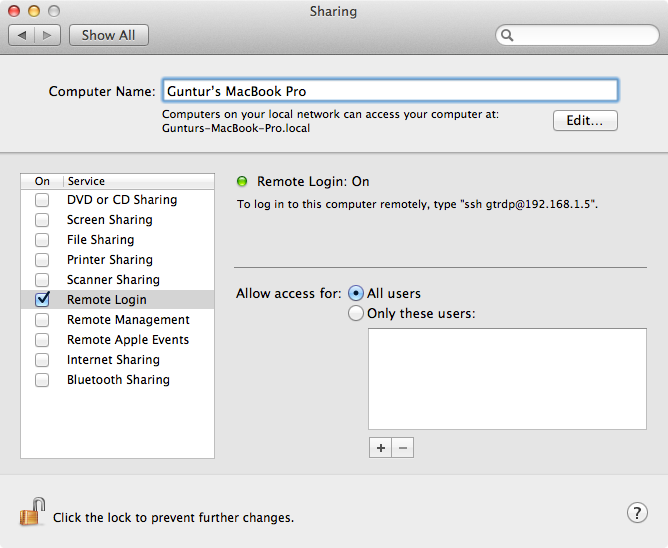
\includegraphics[width=0.8\textwidth]{gambar/mac-sharing}
					    \caption{Konfigurasi SSH pada Mac OS X.}
					    \label{mac-sharing}
					\end{figure}

				\item Peranti XBee

					Setiap peranti XBee yang akan digunakan harus terkonfigurasi terlebih dahulu. Parameter-parameter yang harus terkonfigurasi adalah ATID (alamat dari jaringan/\emph{network ID}), ATMY (alamat peranti itu sendiri), ATDH (\emph{destination address high}), dan ATDL (\emph{destination address low}).

					Proses konfigurasi dilakukan dengan menyambungkan XBee Radio dengan \emph{XBee Explorer USB Board} ke komputer dan menjalankan aplikasi untuk membaca kanal serial, misalnya CoolTerm pada Mac OS X. Setelah CoolTerm dibuka, buka koneksi kanal serial ke XBee dan jalankan perintah dengan format:
					\begingroup
					    \fontsize{10pt}{12pt}\selectfont
					    \begin{verbatim}
							+++		#masuk ke AT Mode
							ATID <id jaringan>
							ATMY <alamat dari zigbee>
							ATDH <destination high>
							ATDL <destination low>
							ATWR 	#tulis ke non volatile memory
					    \end{verbatim}  
					\endgroup

					Contoh perintahnya adalah:
					\begingroup
					    \fontsize{10pt}{12pt}\selectfont
					    \begin{verbatim}
							+++		#masuk ke AT Mode
							ATID 1234
							ATMY 5
							ATDH 0
							ATDL 1
							ATWR 	#tulis ke non volatile memory
					    \end{verbatim}  
					\endgroup
			\end{enumerate}

		\subsection{Pengembangan Aplikasi WSN}
			Langkah selanjutnya yang dilakukan dalam pengembangan adalah pengembangan aplikasi untuk WSN yang terdiri atas aplikasi C yang masing-masing ditujukan untuk IQRF dan XBee. Setelah aplikasi selesai ditulis, kode sesumber kemudian di-\emph{compile} dan diunduh ke dalam WSN.

			\begin{enumerate}
				\item IQRF

					Peranti IQRF dalam penelitian ini ada dua jenis, begitu pula aplikasi/peranti lunak yang tertanam di dalamnya. Aplikasi tersebut adalah \emph{Sink} dan \emph{Node}. Aplikasi \emph{Sink} akan ditanamkan pada koordinator dari IQRF yang terhubung langsung dengan AP melalui kabel USB dan jumlahnya hanya satu. Sedangkan aplikasi \emph{Node} akan ditanamkan pada sensor-sensor IQRF yang akan saling membentuk jaringan jala (\emph{mesh network}) dan jumlahnya lebih dari satu.

					Aplikasi \emph{Sink} lebih ditekankan pada pembentukan ikatan (\emph{bond}) antara koordinator dan sensor-sensor, pengendalian sensor-sensor, serta pengakuisisian data dari masing-masing sensor.

					Sedangkan aplikasi \emph{Node} lebih bersifat pasif karena hanya akan merespon perintah-perintah yang akan dikirimkan oleh koordinator, seperti pembentukan ikatan dan pembacaan temperatur.

					Data yang akan diakuisisi dari masing-masing sensor adalah temperatur yang terbaca di masing-masing sensor.

					Aplikasi yang digunakan adalah hasil \emph{fork} dari aplikasi iHome yang dikembangkan oleh \cite{widyawan2012ihome} yang fiturnya sebenarnya tidak terbatas hanya pada pembacaan temperatur sekitar.

				\item XBee

					Sama seperti IQRF, peranti XBee terdiri dari dua jenis peranti, yaitu koordnator dan sensor-sensor. Koordinator bertugas menyala dan matikan relay-relay yang terdapat di masing-masing sensor sesuai permintaan pengguna.

					Koordinator tersusun atas \emph{XBee 802.15.4 Radios (Series 1)} yang tertanam pada \emph{XBee Explorer USB Board} dan terkoneksi langsung dengan AP dengan kabel USB.

					Sedangkan sensornya terdiri dari tiga bagian, yaitu \emph{XBee 802.15.4 Radios (Series 1)}, \emph{2 channel Relay Shield For Arduino (With XBee/BTBee interface)}, dan Arduino Uno. Ketiga bagian tersebut saling terhubung dengan pin-pin yang tersedia.

					XBee pada hakikatnya hanya sebatas peranti komunikasi antara AP dengan relay-relay yang tersedia, sehingga pemrograman teletak pada masing-masing Arduino pada relay. Bahasa yang digunakan adalah bahasa C (Arduino). Aplikasi yang dikembangkan akan menunggu perintah dari AP untuk menyala dan matikan relay.

			\end{enumerate}

		\subsection{Pengembangan Aplikasi Python}
			Aplikasi Python adalah jantung dari penelitian ini karena menghubungkan aplikasi berbasis web dengan peranti-peranti IQRF dan XBee.	Aplikasi terdiri dari tiga bagian yang ditujukan untuk penggunaan berbeda, yaitu komunikasi dengan sensor IQRF, XBee, dan profil untuk automatisasi.

			\begin{enumerate}
				\item IQRF

					Aplikasi Python IQRF memiliki kemampuan untuk melakukan \emph{bonding} antara koordinator dan sensor, dan pembacaan temperatur pada sensor dengan ID tertentu.

					Diagram alir dari aplikasi berikut dapat dilihat pada Gambar \ref{python-iqrf}.

					\begin{figure}[H]
					  \centering
					    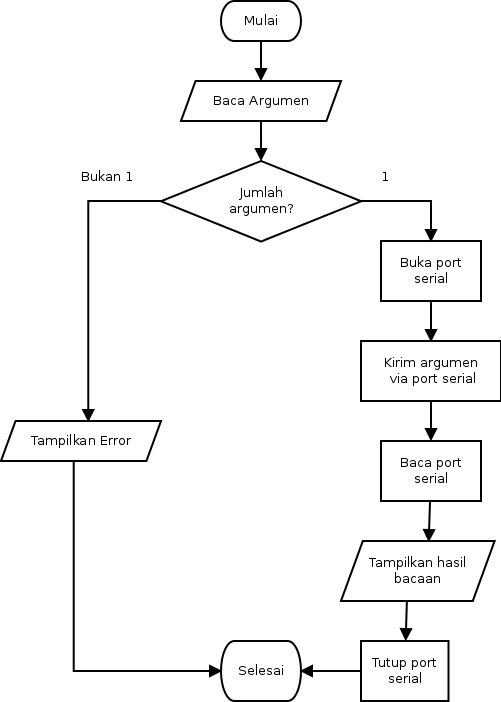
\includegraphics[width=0.6\textwidth]{gambar/python-iqrf}
					    \caption{Diagram alir aplikasi Python untuk IQRF.}
					    \label{python-iqrf}
					\end{figure}

					Aplikasi dijalankan dengan menjalankan format perintah berikut pada \emph{terminal console}:
					\begingroup
					    \fontsize{10pt}{12pt}\selectfont
					    \begin{verbatim}
							$ python iqrf.py <perintah><ID node>
					    \end{verbatim}  
					\endgroup

					Aplikasi ini berjalan dalam bentuk CLI dan membutuhkan satu parameter, yaitu perintah yang langsung disambung dengan ID node tanpa spasi. Perintah yang tersedia yaitu membaca gemperatur pada node ID tertentu (g), \emph{bonding} node ID tertentu (b), \emph{unbonding} node ID tertentu (u).

					Sehingga contoh penggunaan aplikasi pada \emph{terminal console}:
					\begingroup
					    \fontsize{10pt}{12pt}\selectfont
					    \begin{verbatim}
							$ python iqrf.py g3
					    \end{verbatim}  
					\endgroup
					Perintah di atas adalah perintah untuk membaca temperatur pada node ID 3.

				\item XBee

					Aplikasi Python XBee memiliki kemampuan untuk menyala dan matikan relay pada peranti tertentu dan membaca status relay pada peranti tertentu, apakah relay tersebut sedang menyala atau mati.

					Diagram alir dari aplikasi berikut dapat dilihat pada Gambar \ref{python-xbee}.

					\begin{figure}[H]
					  \centering
					    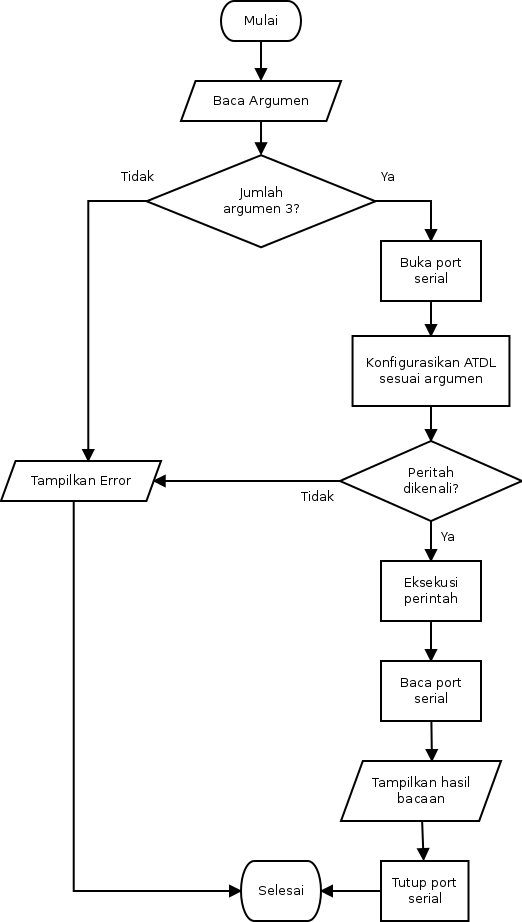
\includegraphics[width=0.6\textwidth]{gambar/python-xbee}
					    \caption{Diagram alir aplikasi Python untuk menangani peranti XBee.}
					    \label{python-xbee}
					\end{figure}

					Aplikasi dijalankan dengan menjalankan format perintah berikut pada \emph{terminal console}:
					\begingroup
					    \fontsize{10pt}{12pt}\selectfont
					    \begin{verbatim}
							$ python xbee.py <perintah> <ATMY peranti> <ID relay>
					    \end{verbatim}  
					\endgroup

					Aplikasi ini berjalan dalam bentuk CLI dan membutuhkan tiga parameter, yaitu perintah, alamat peranti (ATMY), dan ID relay (terdapat dua relay di tiap peranti). Perintah yang tersedia yaitu menyalakan relay, `on', mematikan relay, `off', dan membaca status relay, `status'.

					Sehingga contoh penggunaan aplikasi pada \emph{terminal console}:
					\begingroup
					    \fontsize{10pt}{12pt}\selectfont
					    \begin{verbatim}
							$ python iqrf.py status 2 1
					    \end{verbatim}  
					\endgroup
					Perintah di atas akan membaca status (on/off) dari relay 1 pada peranti dengan alamat (ATMY) 2 dan menampilkannya pada layar dalam karakter `H' (menyala) atau `L' (mati).

				\item \emph{Profile}

					Aplikasi ini memanfaatkan aplikasi \emph{at} pada Linux yang dapat menjalankan perintah tertentu di \emph{terminal console} pada waktu tertentu. Dengan aplikasi ini, pengguna dapat menyala-matikan relay pada waktu tertentu. Jika hal ini dikombinasikan dengan bacaan temperatur dari sensor IQRF, maka pengguna dapat menyala-matikan relay tertentu pada saat temperatur pada sensor IQRF node tertentu mencapai suhu tertentu, dan juga bisa hanya terjadi saat waktu tertentu.

					Diagram alir dari aplikasi berikut dapat dilihat pada Gambar \ref{python-profile}.

					\begin{figure}[H]
					  \centering
					    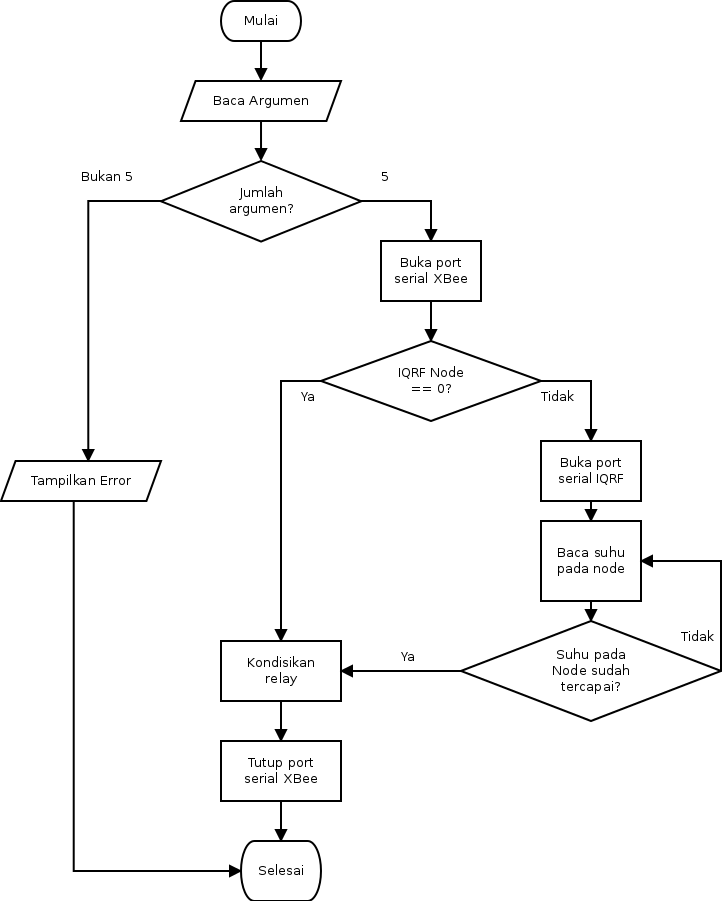
\includegraphics[width=0.8\textwidth]{gambar/python-profile}
					    \caption{Diagram alir aplikasi Python untuk menyala-matikan lampu pada kondisi tertentu.}
					    \label{python-profile}
					\end{figure}

			\end{enumerate}

		\subsection{Pengembangan Aplikasi Berbasis Web}
			Aplikasi web untuk mengendalikan sensor-sensor IQRF dan XBee dibangun dengan PHP dan basis data MySQL. Aplikasi ini dibangun tanpa menggunakan \emph{framework} karena aplikasi ini tergolong tidak terlalu rumit, aplikasi ini hanya memliki lima halaman utama seperti terlihat pada sitemap Gambar \ref{sitemap}. Penggunaan \emph{framework} juga akan memakan sumber daya komputasi sedikit lebih banyak, padahal aplikasi ini akan diimplementasikan pada sebuah AP yang memiliki tingkat komputasi yang rendah.

			Antarmuka yang dikembangkan adalah hasil \emph{fork} dari \emph{template} halaman administrator buatan Vince G. Antarmuka ditulis menggunakan HTML5 dan CSS3, dengan tambahan pemrograman JavaScript pada sisi klien agar menambah interaktivitas. Pustaka Bootstrap digunakan untuk membuat halaman web menjadi responsif, sehingga dapat menyesuaikan diri secara otomatis sesuai dengan ukuran layar. Pustaka jQuery digunakan untuk membantu pemrograman di sisi klien.

			Kode sesumber untuk aplikasi berbasis web ditulis dengan bantuan Sublime Text 3.
			
			Peta situs dari aplikasi berbasis web yang dikembangkan dapat dilihat pada Gambar \ref{sitemap}.
			
			\begin{figure}[H]
			  \centering
			    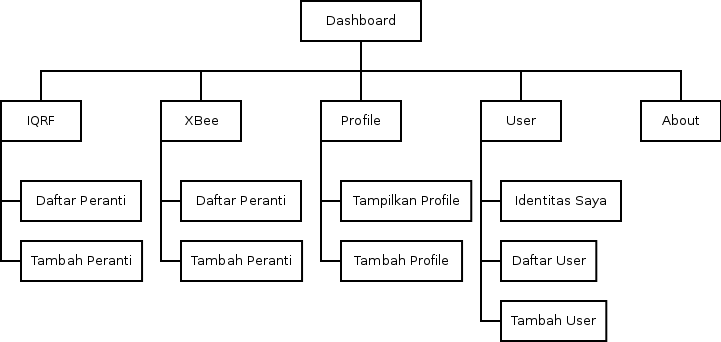
\includegraphics[width=0.8\textwidth]{gambar/sitemap}
			    \caption{Peta situs aplikasi web.}
			    \label{sitemap}
			\end{figure}

			Total halaman utama dari situs ada enam halaman, seperti dapat dilihat pada Gambar \ref{sitemap} dengan tambahan halaman login, halaman yang harus diakses sebelum pengguna dapat masuk ke dalam sistem. Empat halaman utama mempunyai halaman anak yang secara garis besar ditujukan untuk melihat, menghapus dan menambah peranti, profil, atau pengguna.

			Basis data yang dikembangkan tergolong sederhana karena hanya dimaksudkan untuk menyimpan data-data yang sifatnya kecil, seprti tampak pada Gambar \ref{erd}.

			\begin{figure}[H]
			  \centering
			    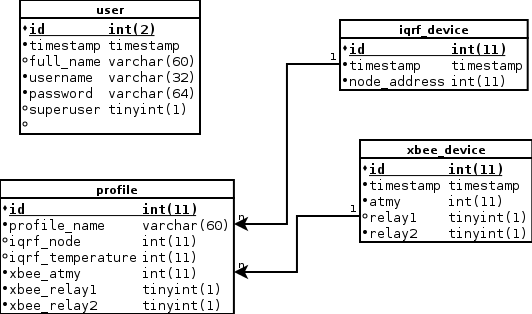
\includegraphics[width=0.6\textwidth]{gambar/erd}
			    \caption{\emph{Entity Relationship Diagram} dari basis data untuk aplikasi web.}
			    \label{erd}
			\end{figure}

			Seperti yang terpampang pada Gambar \ref{erd}, basis data terdiri atas empat tabel. Relasi yang ada pada basis data hanya relasi tabel \emph{iqrf\_device} dengan \emph{profile} dan \emph{xbee\_device} dengan \emph{profile}.

			Sedangkan diagram alir untuk menambah peranti IQRF dan XBee dijelaskan pada Gambar \ref{add-iqrf} dan Gambar \ref{add-xbee}.

			\begin{figure}[H]
			  \centering
			    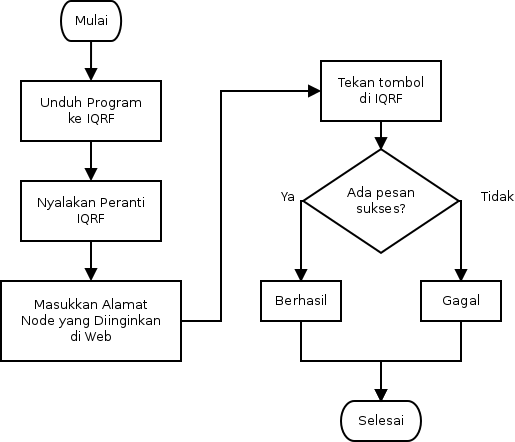
\includegraphics[width=0.6\textwidth]{gambar/add-iqrf}
			    \caption{Diagram Alir Penambahan Peranti IQRF ke Aplikasi.}
			    \label{add-iqrf}
			\end{figure}

			\begin{figure}[H]
			  \centering
			    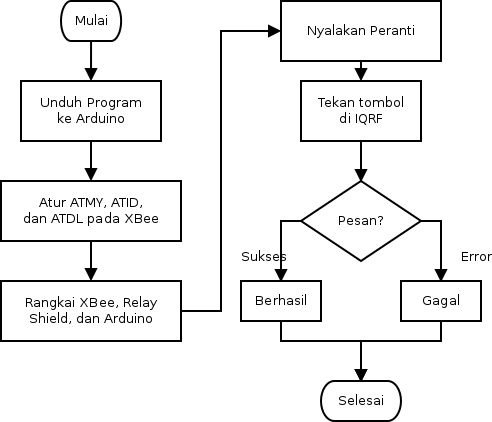
\includegraphics[width=0.6\textwidth]{gambar/add-xbee}
			    \caption{Diagram Alir Penambahan Peranti XBee ke Aplikasi.}
			    \label{add-xbee}
			\end{figure}

			Penambahan peranti IQRF mengharuskan pengguna untuk menekan tombol yang ada pada sensor IQRF, sedangkan penambahan peranti XBee tidak mengharuskan pengguna untuk menekan tombol atau mengintervensi perangkat keras XBee.

		\subsection{Evaluasi dan Perbaikan}
			Evaluasi dilakukan dengan mengujikan semua fitur yang dimiliki oleh aplikasi. Jika terdapat kesalahan, maka dilacak dimanakah letak kesalahan berada, apakah pada aplikasi berbasis web, aplikasi Python, atau aplikasi C pada sensor.

			Masalah yang timbul adalah saat akan merevisi aplikasi yang sudah terlanjur tertanam pada AP karena AP, dengan sistem operasi OpenWRT, tidak memiliki aplikasi teks editor yang mumpuni untuk melakukan pengeditan kode sesumber dengan nyaman. Oleh karena itu, seluruh kode sesumber tetap berada pada komputer agar tetap bisa dibuka dengan Sublime Text 3, namun AP me-\emph{mount}-nya dengan bantuan SSHFS sehingga seolah-olah kode sesumber tersebut berada dalam dua tempat dan saling tersinkronisasi.

			Untuk melakukan \emph{mounting} pada AP, menggunakan perintah:
			\begingroup
			    \fontsize{10pt}{12pt}\selectfont
			    \begin{verbatim}
					# sshfs /direktori/pada/ap <user>@<alamat IP>:/direktori/pada/komputer
			    \end{verbatim}  
			\endgroup

			Contoh penggunaan perintah tersebut:
			\begingroup
			    \fontsize{10pt}{12pt}\selectfont
			    \begin{verbatim}
					# sshfs /www/web/ gtrdp@192.168.1.1:/var/www/web/
			    \end{verbatim}  
			\endgroup
			

		\subsection{\emph{Screenshot} Aplikasi}
			Bagian ini menampilkan beberapa \emph{screenshot} dari aplikasi web yang dikembangkan.

			Halaman pertama yang akan terbuka setelah pengguna melakukan \emph{log in} adalah halaman \emph{dashboard} seperti yang dapat dilihat pada Gambar \ref{dashboard}. Tampilan halaman web akan menyesuaikan dengan layar pengguna karena halaman tersebut didesain responsif.

				\begin{figure}[H]
					\begin{subfigure}[b]{\textwidth}
						\centering
					    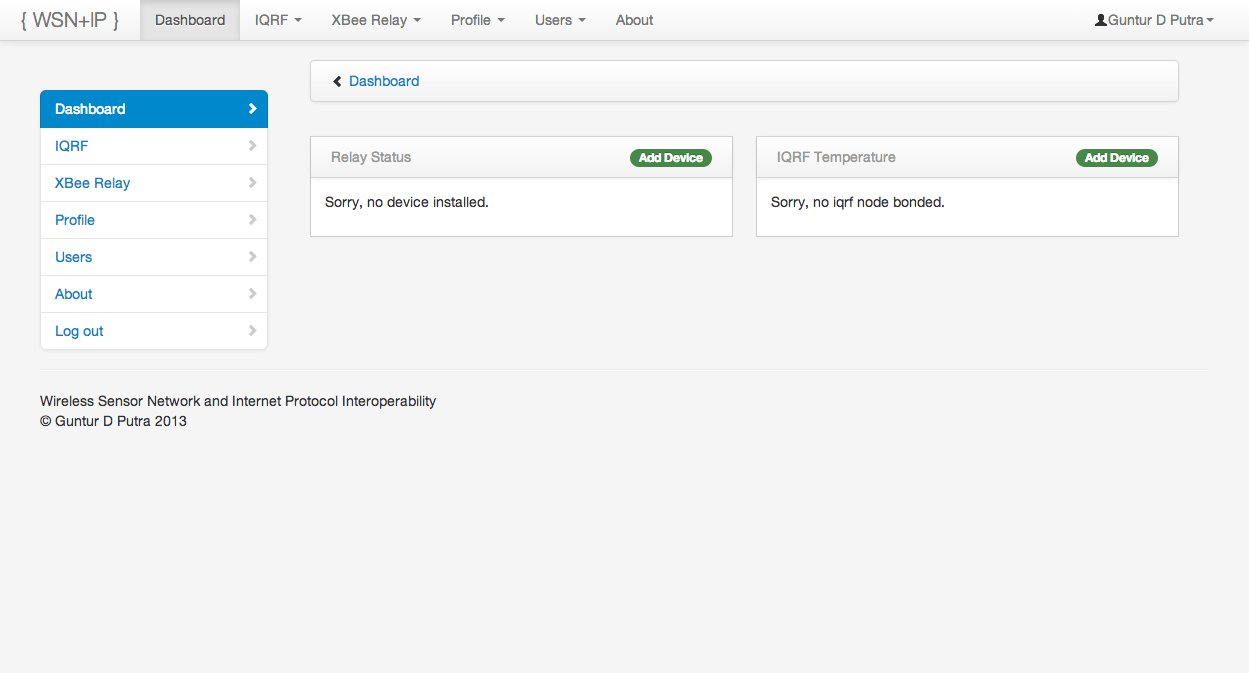
\includegraphics[width=0.9\textwidth]{gambar/dashboard}
					    \caption{Dibuka pada layar komputer.}
					    \label{dashboard-full-page}
					\end{subfigure}
					 ~
					\begin{subfigure}[b]{\textwidth}
						\centering
					    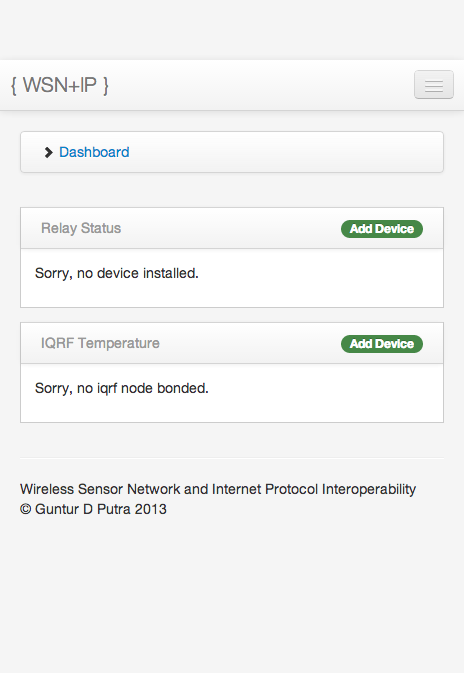
\includegraphics[width=0.3\textwidth]{gambar/dashboard-small}
					    \caption{Dibuka di layar ponsel yang kecil.}
					    \label{dashboard-small}
					\end{subfigure}
					\caption{Halaman \emph{dashboard} saat belum ada peranti terpasang.}
					\label{dashboard}
				\end{figure}

			Seperti dapat dilihat pada Gambar \ref{dashboard-small}, ukuran layar akan menjadi lebih kecil jika dibanding dengan Gambar \ref{dashboard-full-page} karena halaman dibuka pada ponsel cerdas yang memiliki ukuran layar lebih kecil dari komputer.

			Aplikasi mempunyai halaman untuk menambahkan peranti IQRF, sehingga pengguna dapat menambahkan peranti IQRF baru ke dalam sistem menggunakan halaman ini. Gambar \ref{iqrf-add} menunjukkan halaman untuk menambahkan peranti IQRF.

				\begin{figure}[H]
				  \centering
				    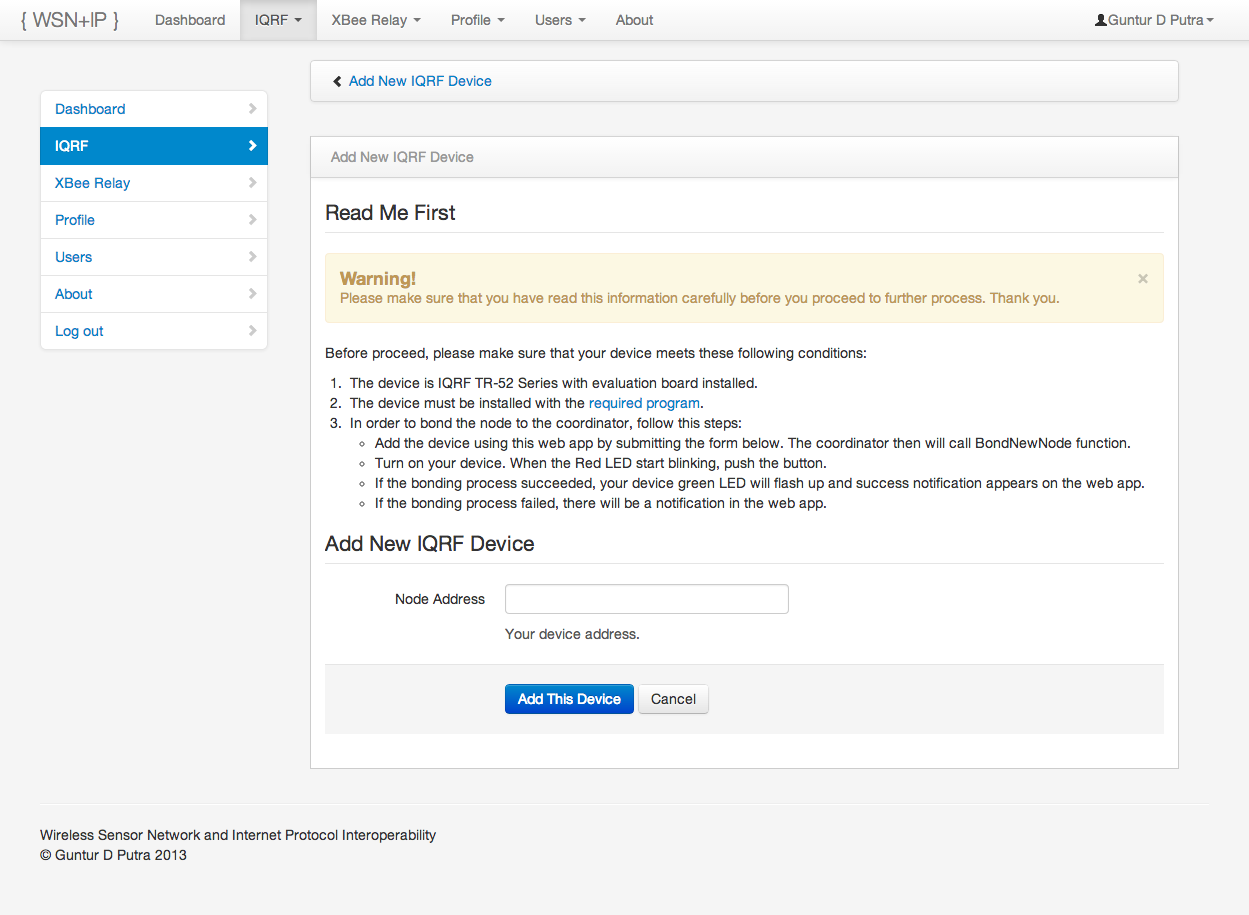
\includegraphics[width=0.9\textwidth]{gambar/iqrf-add}
				    \caption{Halaman untuk menambahkan peranti IQRF.}
				    \label{iqrf-add}
				\end{figure}

			Seperti dapat dilihat pada Gambar \ref{iqrf-add}, pengguna diharuskan untuk memasukkan alamat \emph{node} dari IQRF yang akan ditambahkan. Alamat tersebut adalah bilangan bulat dari dua dan tidak boleh menggunakan alamat yang sudah terpasang pada sistem. Pada bagian atas halaman, terdapat langkah-langkah yang harus diikuti pengguna untuk menambahkan peranti IQRF baru.

			Seperti peranti IQRF, aplikasi juga menyediakan halaman khusus untuk menambahkan peranti XBee, seperti yang dapat dilihat pada Gambar \ref{xbee-add}.

				\begin{figure}[H]
				  \centering
				    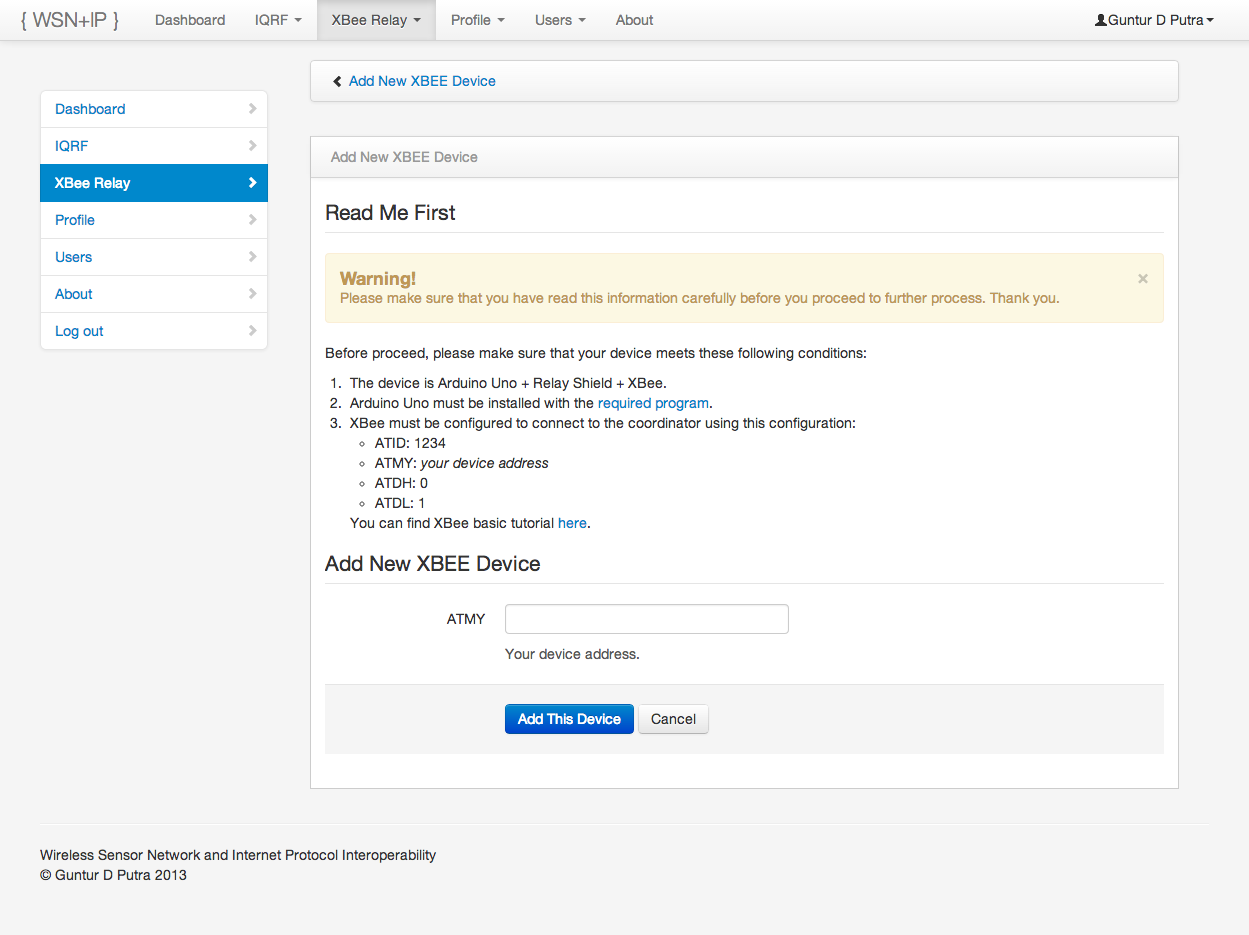
\includegraphics[width=0.9\textwidth]{gambar/xbee-add}
				    \caption{Halaman untuk menambahkan peranti XBee.}
				    \label{xbee-add}
				\end{figure}

			Pengguna juga diharuskan untuk memasukkan alamat ATMY dari XBee yang akan ditambahkan, seperti cara menambahkan peranti IQRF. Pada bagian atas halaman, terdapat langkah-langkah yang harus diikuti pengguna untuk menambahkan peranti XBee baru.

			Saat peranti sudah ditambahkan melalui halaman-halaman yang sudah dijelaskan sebelumnya, halaman \emph{dashboard} akan berubah, seperti yang tergambar pada Gambar \ref{dashboard-full-device}. Halaman ini masih bersifat responsif, sehingga akan menyesuaikan dengan layar di mana halaman tertampil.

				\begin{figure}[H]
				  \begin{subfigure}[b]{\textwidth}
				  \centering
				    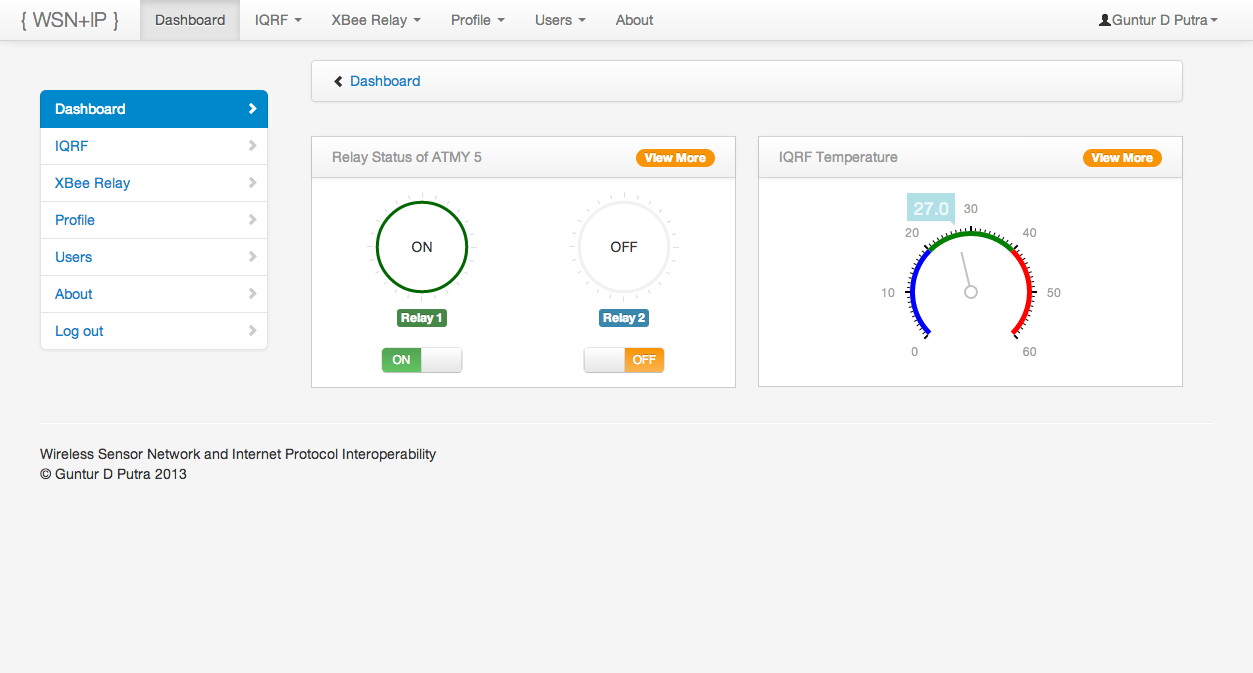
\includegraphics[width=0.9\textwidth]{gambar/dashboard-full}
				    \caption{Dibuka pada layar komputer.}
				    \label{dashboard-full}
				  \end{subfigure}
				~
				  \begin{subfigure}[b]{\textwidth}
				  \centering
				    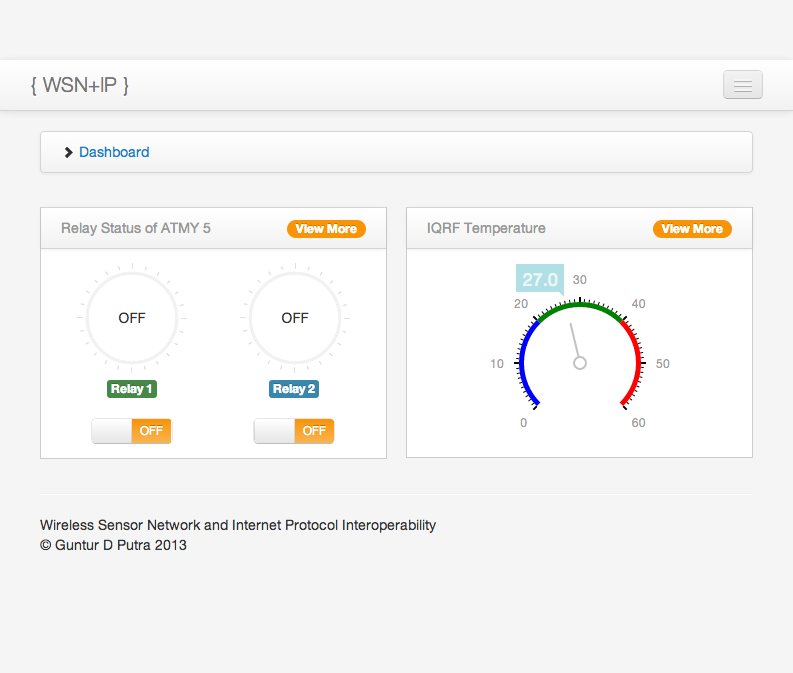
\includegraphics[width=0.6\textwidth]{gambar/dashboard-full-small}
				    \caption{Dibuka pada layar ponsel yang kecil.}
				    \label{dashboard-full-small}
				  \end{subfigure}
				  \caption{Halaman \emph{dashboard} saat peranti sudah terpasang.}
				  \label{dashboard-full-device}
				\end{figure}

			Pada saat halaman dibuka pada layar yang kecil, maka perbedaan yang signifikan adalah hilangnya \emph{sidebar} dan mengecilnya \emph{navigation bar} seperti yang dapat dilihat pada Gambar \ref{dashboard-full} dan \ref{dashboard-full-small}.

			Berapapun banyaknya sensor IQRF atau XBee yang terpasang, halaman \emph{dashboard} tetap akan menampilkan satu peranti saja, yaitu peranti yang pertama kali terpasang. Jika penggune ingin melihat semua sensor yang terpasang, pengguna dapat membuka halaman khusus untuk melihat semua sensor IQRF yang terpasang, seperti yang ditunjukkan pada Gambar \ref{iqrf-list}.

				\begin{figure}[H]
				  \centering
				    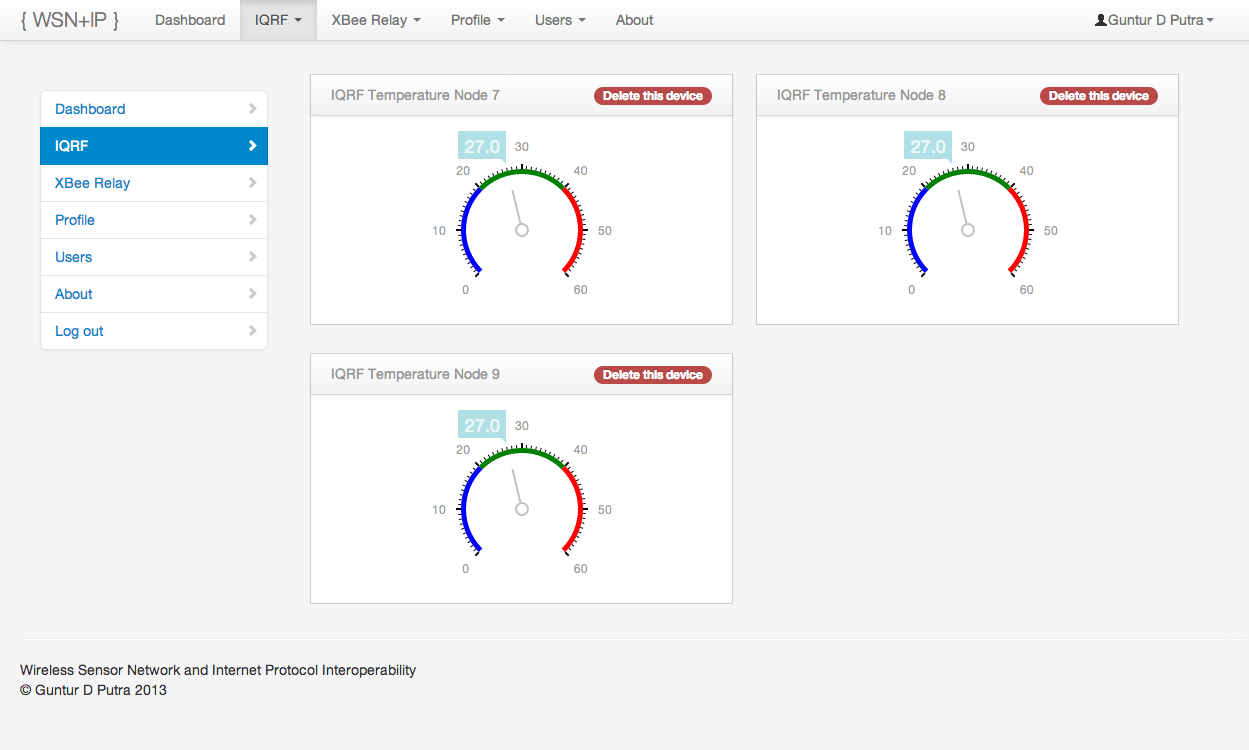
\includegraphics[width=0.9\textwidth]{gambar/iqrf-list}
				    \caption{Halaman daftar peranti IQRF yang terpasang.}
				    \label{iqrf-list}
				\end{figure}

			Pada Gambar \ref{iqrf-list} tertampil tiga buah termometer digital yang masing-masing menampilkan hasil bacaan temperatur dari masing-masing sensor IQRF. Perubahan suhu dapat dilihat secara langsung.

			Pengguna juga dapat melihat semua peranti XBee yang terpasang dengan halaman khusus yang tertera pada Gambar \ref{xbee-list}. Halaman ini akan menampilkan semua peranti XBee yang terdaftar pada aplikasi.

				\begin{figure}[H]
				  \centering
				    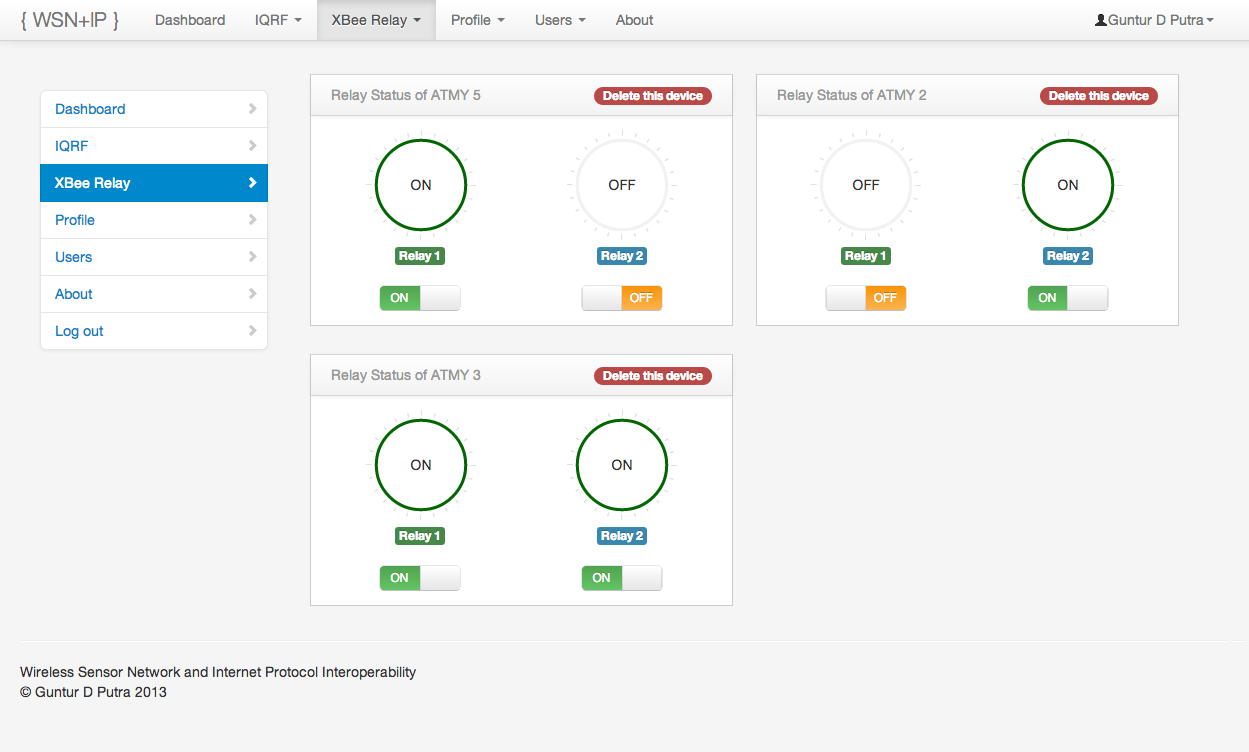
\includegraphics[width=0.9\textwidth]{gambar/xbee-list}
				    \caption{Halaman daftar peranti XBee yang terpasang.}
				    \label{xbee-list}
				\end{figure}

			Seperti yang dapat dilihat pada Gambar \ref{xbee-list}, terdapat tiga peranti XBee yang terdaftar pada aplikasi. Melalui halaman ini, pengguna dapat memati-nyalakan sensor dengan meng-klik saklar yang diinginkan. Dibutuhkan sekitar dua sampai tiga detik untuk menyalakan relay.

			Seperti yang sudah dijelaskan, aplikasi mendukung profil guna otomatisasi tugas-tugas tertentu. Jika pengguna mengiginkan untuk menambahkan profil tertentu, tersedia halaman khusus seperti yang terlihat pada Gambar \ref{profile-add}. Jika suhu yang terbaca di sensor IQRF tertentu mencapai nilai yang diinginkan, maka kondisi relay pada peranti XBee tertentu akan terkonfigurasi seperti yang diinginkan pengguna. Untuk lebih jelasnya bisa dilihat pada Gambar \ref{profile-add}.

				\begin{figure}[H]
				  \centering
				    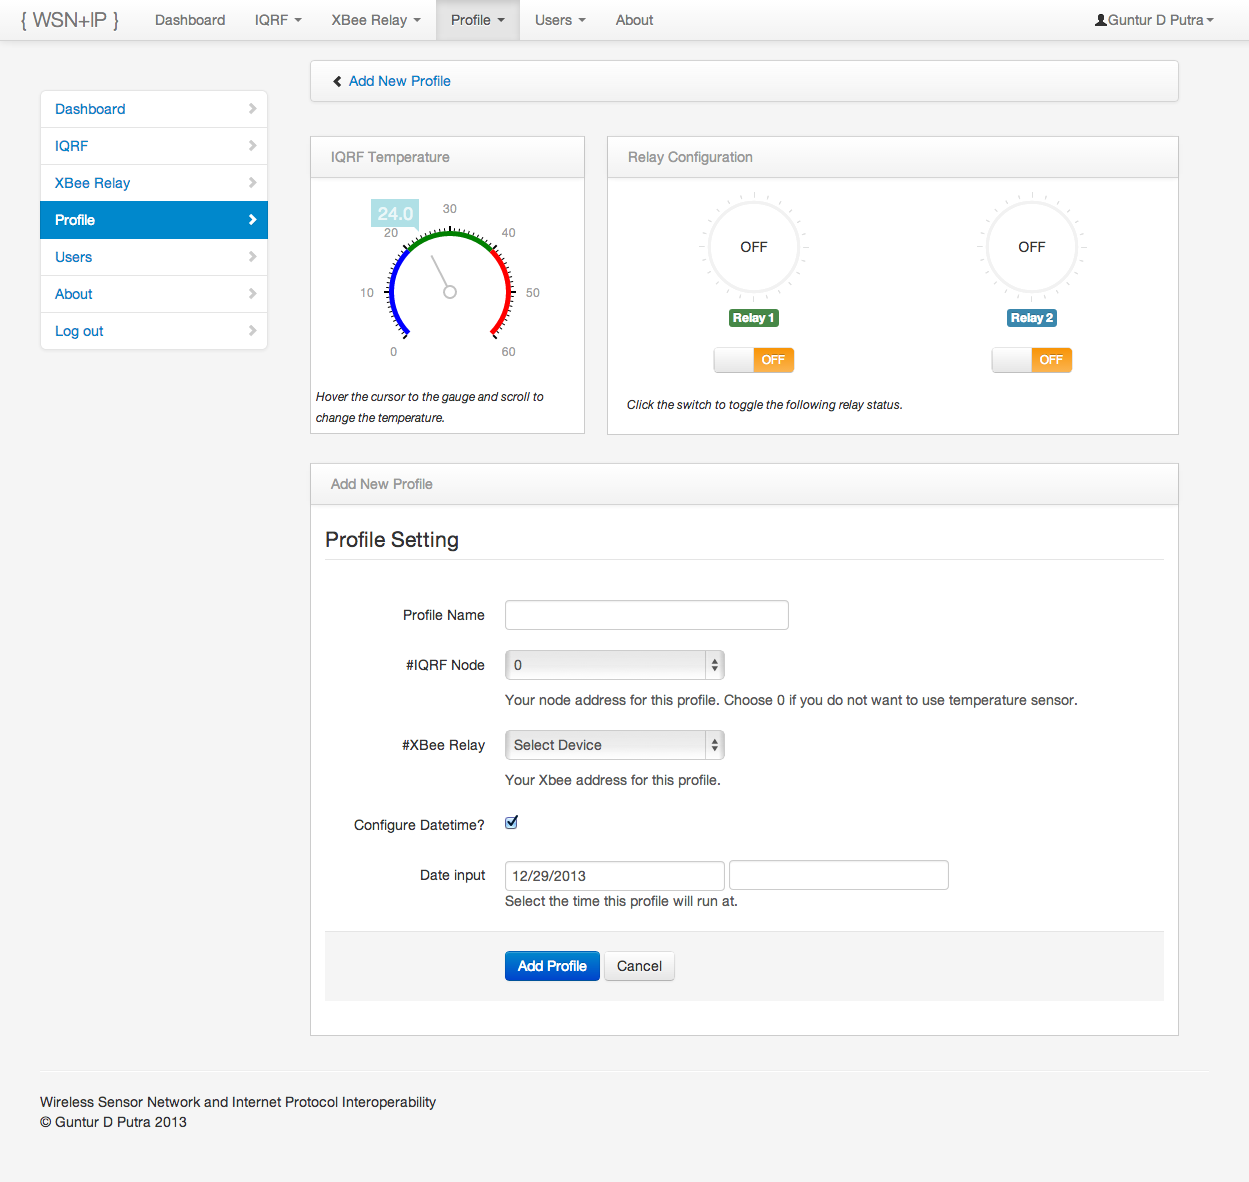
\includegraphics[width=0.9\textwidth]{gambar/profile-add}
				    \caption{Halaman untuk menambahkan profil.}
				    \label{profile-add}
				\end{figure}

			Informasi yang harus dimasukkan ke dalam aplikasi agar pengguna dapat menambahkan profil baru, seperti yang terlihat pada Gambar \ref{profile-add}, adalah:

				\begin{itemize}
					\item temperatur yang diinginkan,
					\item konfigurasi relay saat temperatur tercapai,
					\item nama profil,
					\item alamat sensor IQRF yang diinginkan (pembacaan temperatur),
					\item alamat ATMY peranti XBee yang diinginkan (relay),
					\item dan tanggal dan waktu yang diinginkan.
				\end{itemize}

			Namun jika pengguna hanya ingin menyala-matikan relay XBee pada waktu tertentu, maka pengguna tinggal memilih alamat nol (0) untuk sensor IQRF. Dengan demikian, pembacaan temperatur pada IQRF akan diabaikan.

			Jika pengguna ingin relay XBee terkonfigurasi saat IQRF membaca temperatur tertentu, tanpa memperhatikan tanggal dan waktu, pengguna hanya mencentang \emph{checkbox} yang sudah tersedia. Dengan demikian, profil akan berjalan tanpa memperhatikan waktu tertentu.

			Halaman selanjutnya adalah halaman yang menampilkan semua pengguna yang terdaftar, seperti yang dapat dilihat pada Gambar \ref{user-list}. Namun yang dapat mengakses halaman ini adalah pengguna yang berstatus \emph{administrator}.

				\begin{figure}[H]
				  \centering
				    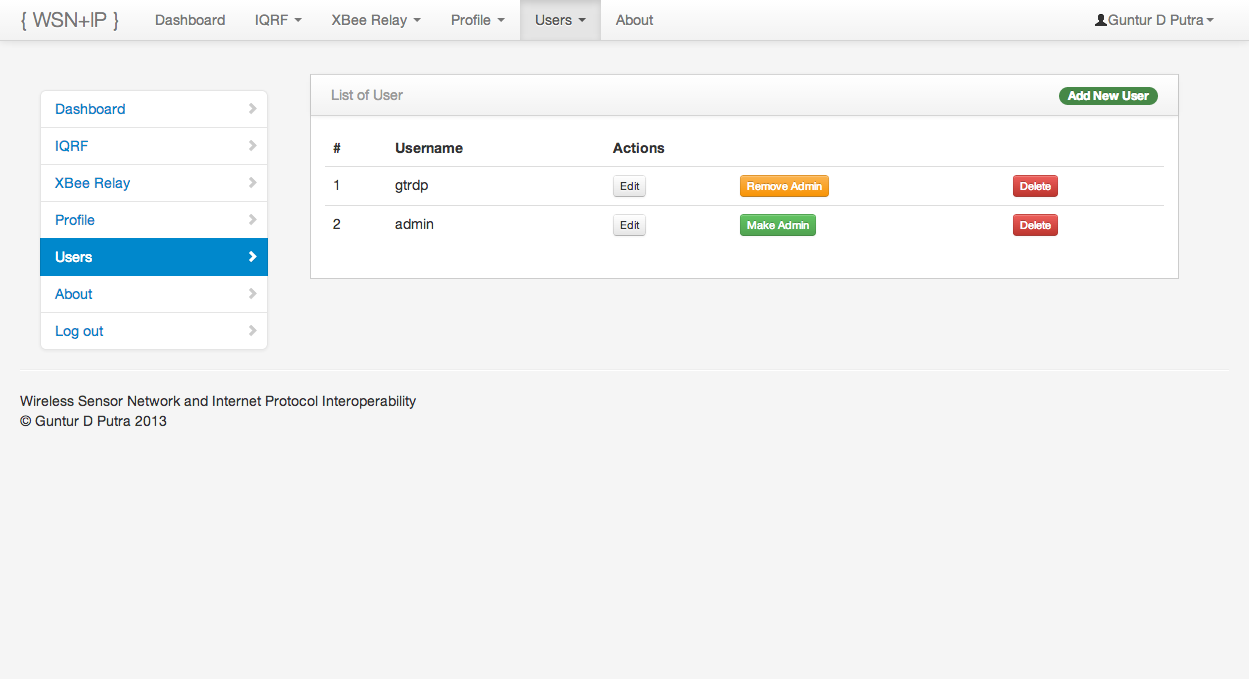
\includegraphics[width=0.9\textwidth]{gambar/user-list}
				    \caption{Halaman yang menampilkan daftar pengguna.}
				    \label{user-list}
				\end{figure}

			Pada halaman ini, terdapat tautan untuk menambahkan pengguna baru, mengedit data pengguna yang sudah terdaftar, menghapus data pengguna, dan menaikkan status pengguna menjadi \emph{administrator} atau menurunkannya.

			Jika pengguna meng-klik tautan untuk menambahkan pengguna baru, maka pengguna akan diarahkan menuju halaman baru seperti yang dapat dilihat pada Gambar \ref{user-add}. Pada halaman ini, pengguna diminta untuk memasukkan informasi-informasi tentang pengguna baru.

				\begin{figure}[H]
				  \centering
				    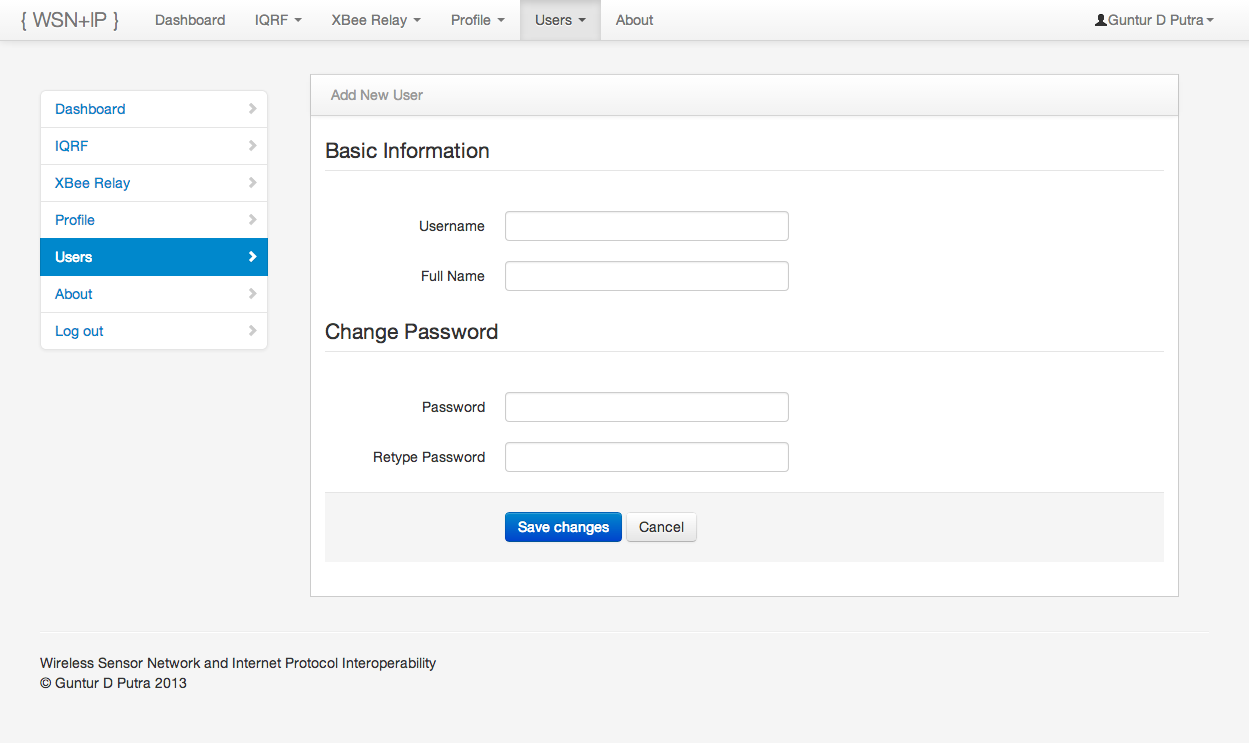
\includegraphics[width=0.9\textwidth]{gambar/user-add}
				    \caption{Halaman untuk menambahkan pengguna baru.}
				    \label{user-add}
				\end{figure}

			Informasi yang harus dimasukkan, seperti yang dapat dilihat pada Gambar \ref{user-add}, antara lain:

				\begin{itemize}
					\item \emph{username} pengguna baru,
					\item nama lengkap pengguna baru,
					\item dan kata sandi pengguna (dua kali).
				\end{itemize}

			Untuk dapat mengakses semua fitur/halaman di atas, pengguna harus \emph{log in} terlebih dahulu. Halaman login dari aplikasi web terlihat pada Gambar \ref{login}.

				\begin{figure}[H]
				  \centering
				    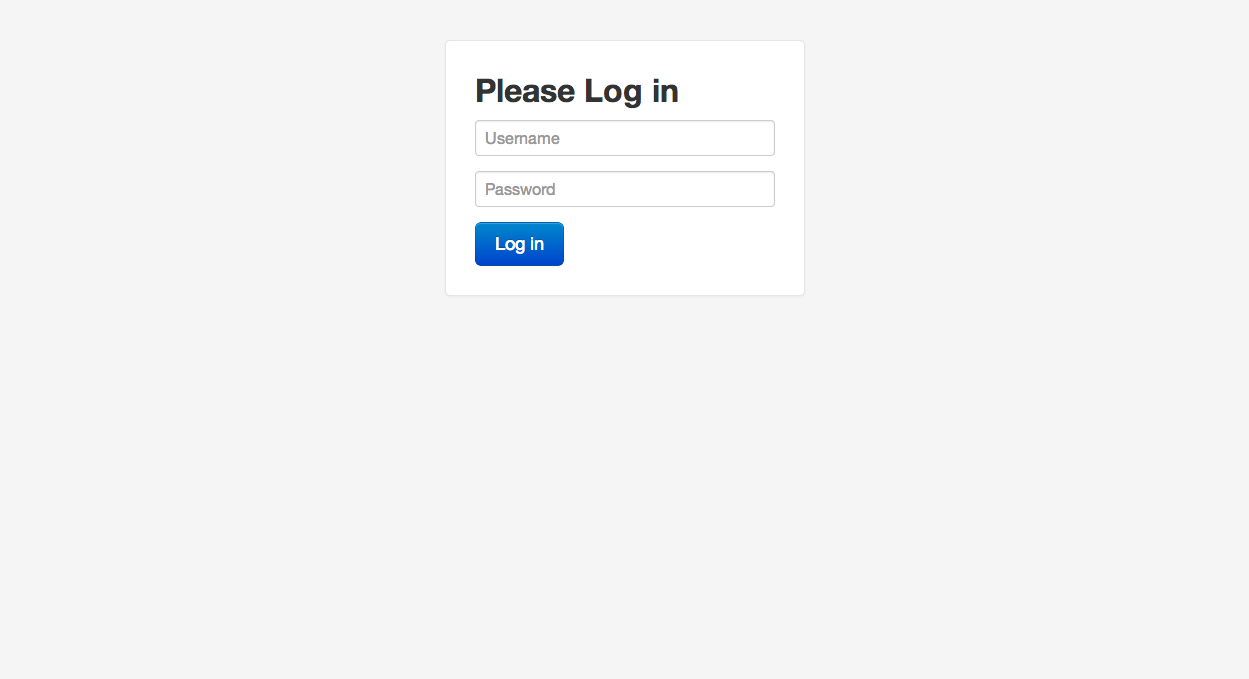
\includegraphics[width=0.9\textwidth]{gambar/login}
				    \caption{Halaman login.}
				    \label{login}
				\end{figure}

			Informasi yang dibutuhkan untuk \emph{log in} hanya \emph{username} atau nama pengguna, dan \emph{password} atau kata sandi.

			Pendekatan yang dilakukan pada aplikasi ini tidak seperti aplikasi web pada umumnya, di mana pengguna dapat mengklik tautan registrasi yang biasanya terdapat pada halaman \emph{log in}. Pendekatan yang dilakukan seperti pada proses \emph{log in} pada komputer. Jadi jika pengguna baru ingin masuk, ia bisa mendaftarkan dirinya melalui pengguna lama yang sudah dapat \emph{log in}, menggunakan halaman yang sudah dijelaskan sebelumnya pada Gambar \ref{user-add}.


		\subsection{Kode Sesumber}
			Kode sesumber dapat diperoleh pada situs GitHub dengan alamat URL \url{https://github.com/gtrdp/wsn-ip-interoperability}. Pada laman tersebut, kode sesumber dapat diunduh dalam format .zip. Dengan bantuan aplikasi git, \emph{project} dari aplikasi ini, lengkap dari aplikasi C, Python, dan Web, dapat di-kloning.


	\section{Analisis Unjuk Kerja Aplikasi}
		Bagian terakhir dari skripsi ini akan ini menjelaskan hal-hal terkait tentang cara perangkaian perangkat keras sehingga dapat difungsikan, instalasi aplikasi ke peranti sehingga sesuai kondisi sesungguhnya, hasil uji coba aplikasi, serta masalah yang dihadapi dan penyelesaiannya.

		\subsection{Instalasi Peranti}
			Perangkat keras pertama yang akan dirakit adalah koordinator IQRF yang tersambung langsung pada AP. Koordinator IQRF ini terdiri atas kabel USB to Serial Prolific, kit pengembangan CK-EVAL-04, dan IQRF TR-52B seperti dapat dilihat pada Gambar \ref{iqrf-coordinator}. Kondisi koordinator sensor IQRF sebelum dirakit dapat dilihat pada Gambar \ref{iqrf-stripped}.

			\begin{figure}[H]
				\begin{subfigure}[b]{\textwidth}
					\centering
				    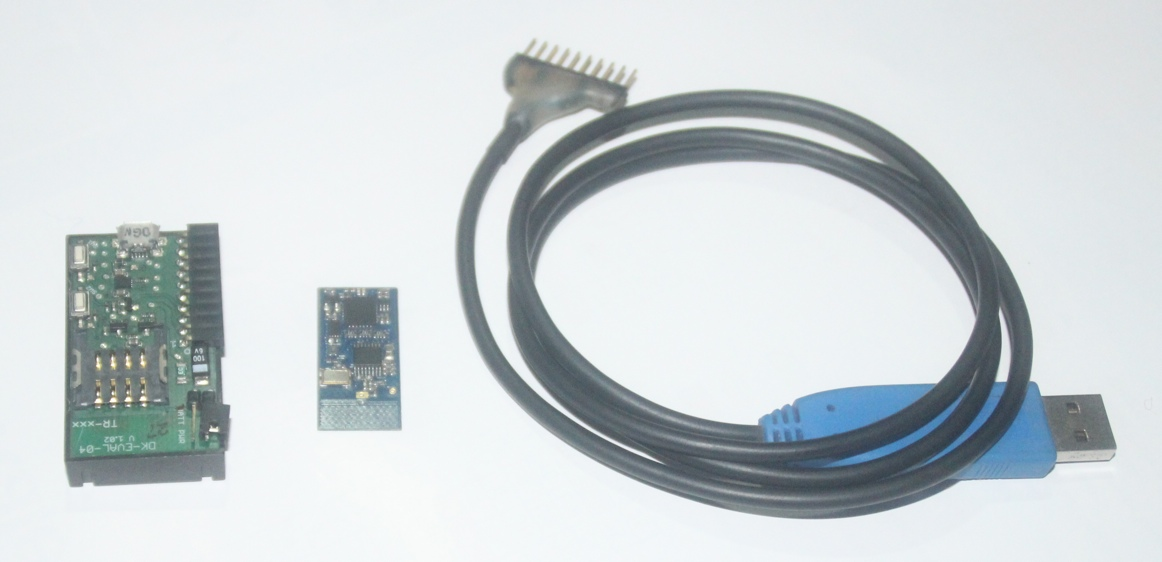
\includegraphics[width=0.7\textwidth]{gambar/iqrf-stripped}
				    \caption{Sebelum dirakit.}
				    \label{iqrf-stripped}
				\end{subfigure}
				 ~
				\begin{subfigure}[b]{\textwidth}
					\centering
				    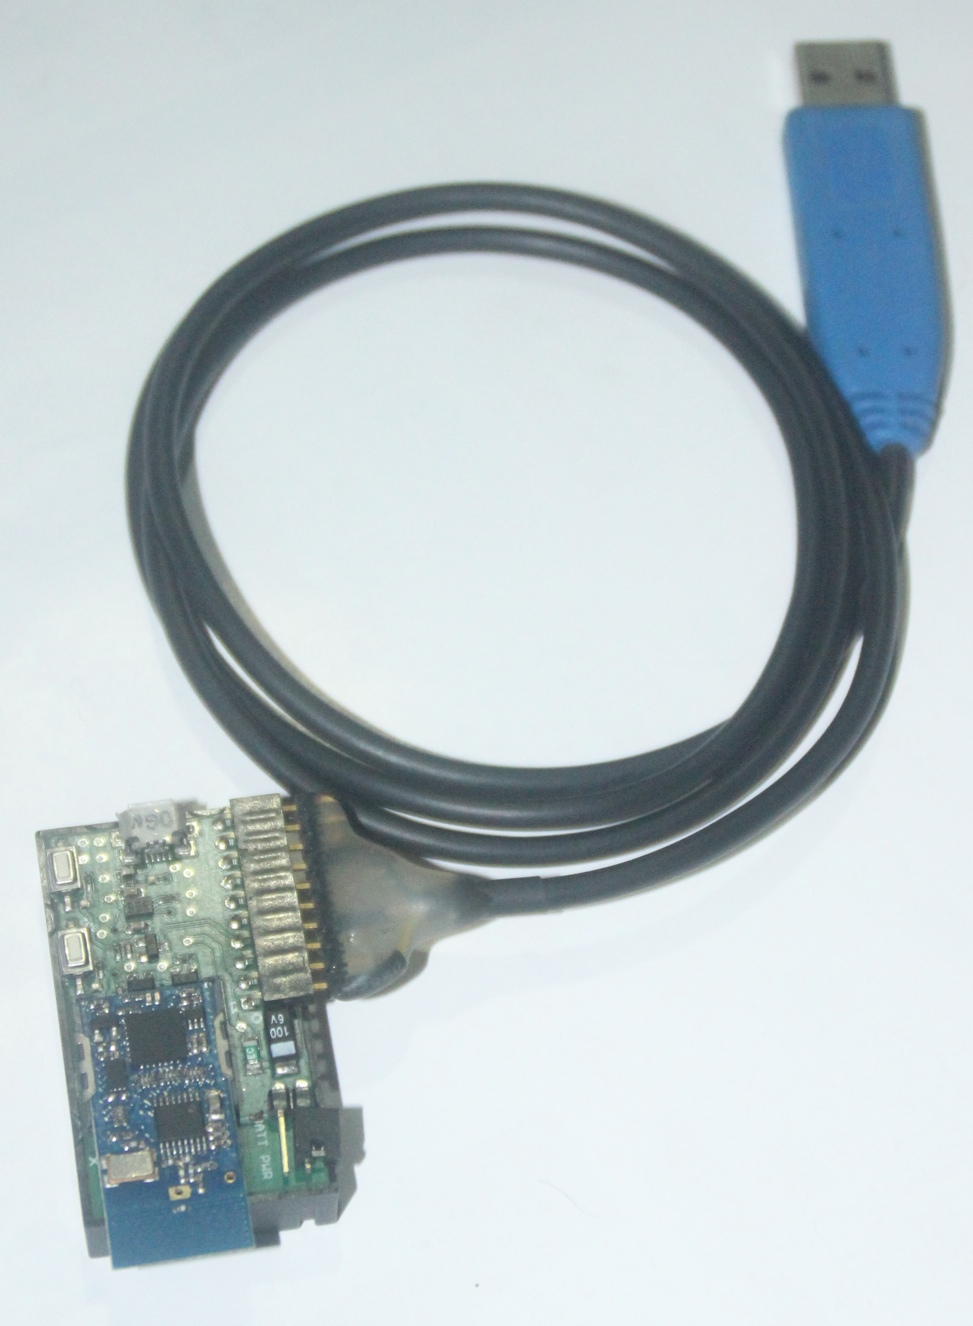
\includegraphics[width=0.5\textwidth]{gambar/iqrf-complete}
				    \caption{Setelah dirakit.}
				    \label{iqrf-complete}
				\end{subfigure}
				\caption{Koordinator sensor IQRF yang akan disambungkan pada AP.}
				\label{iqrf-coordinator}
			\end{figure}

			Kemudian semua bagian disambungkan pada tempatnya. Untuk kabel USB to Serial Prolific, posisi kabel \emph{ground} terpasang pada bagian bawah seperti terlihat pada Gambar \ref{iqrf-complete}.

			Koordinator peranti XBee pada AP terdiri atas \emph{XBee 802.15.4 Radios (Series 1)} dan \emph{XBee Explorer USB Board} yang tersambung pada AP dengan kabel mini-USB seperti dapat dilihat pada Gambar \ref{xbee-sink}.

			\begin{figure}[H]
				\begin{subfigure}[b]{\textwidth}
					\centering
				    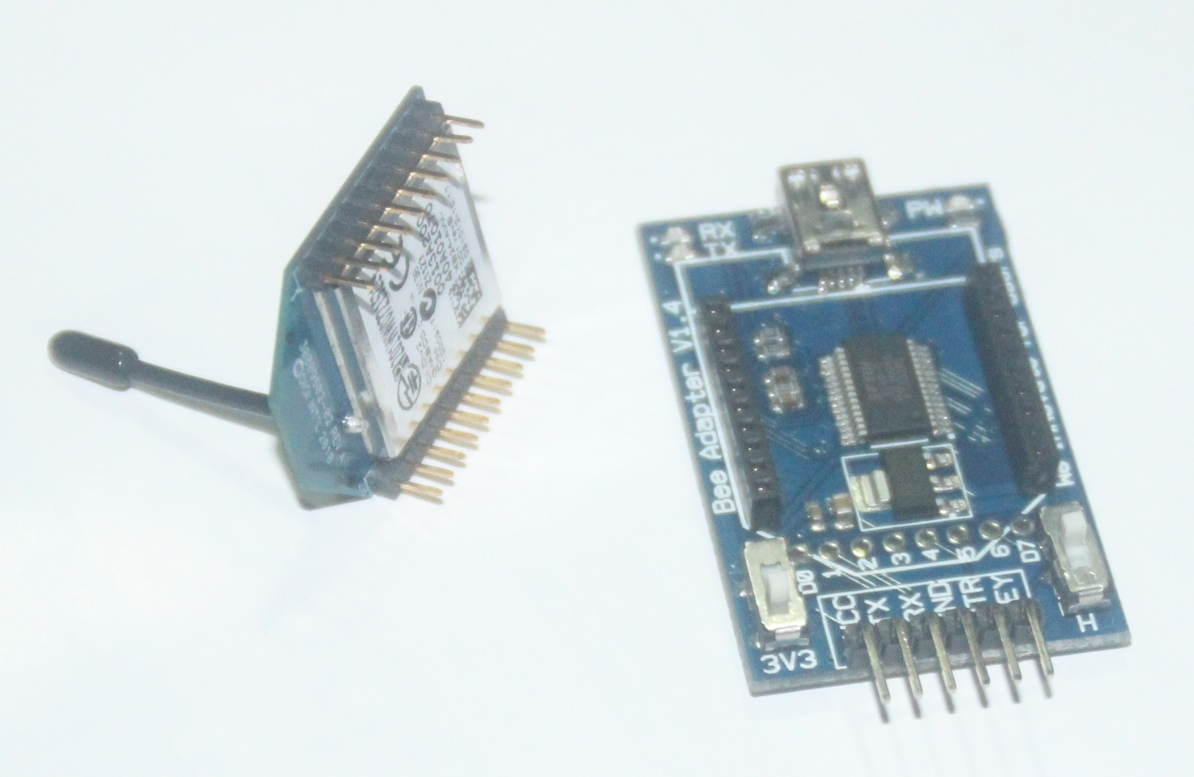
\includegraphics[width=0.5\textwidth]{gambar/xbee-sink-stripped}
				    \caption{Koordinator XBee saat sebelum dirakit.}
				    \label{xbee-sink-stripped}
				\end{subfigure}
				 ~
				\begin{subfigure}[b]{\textwidth}
					\centering
				    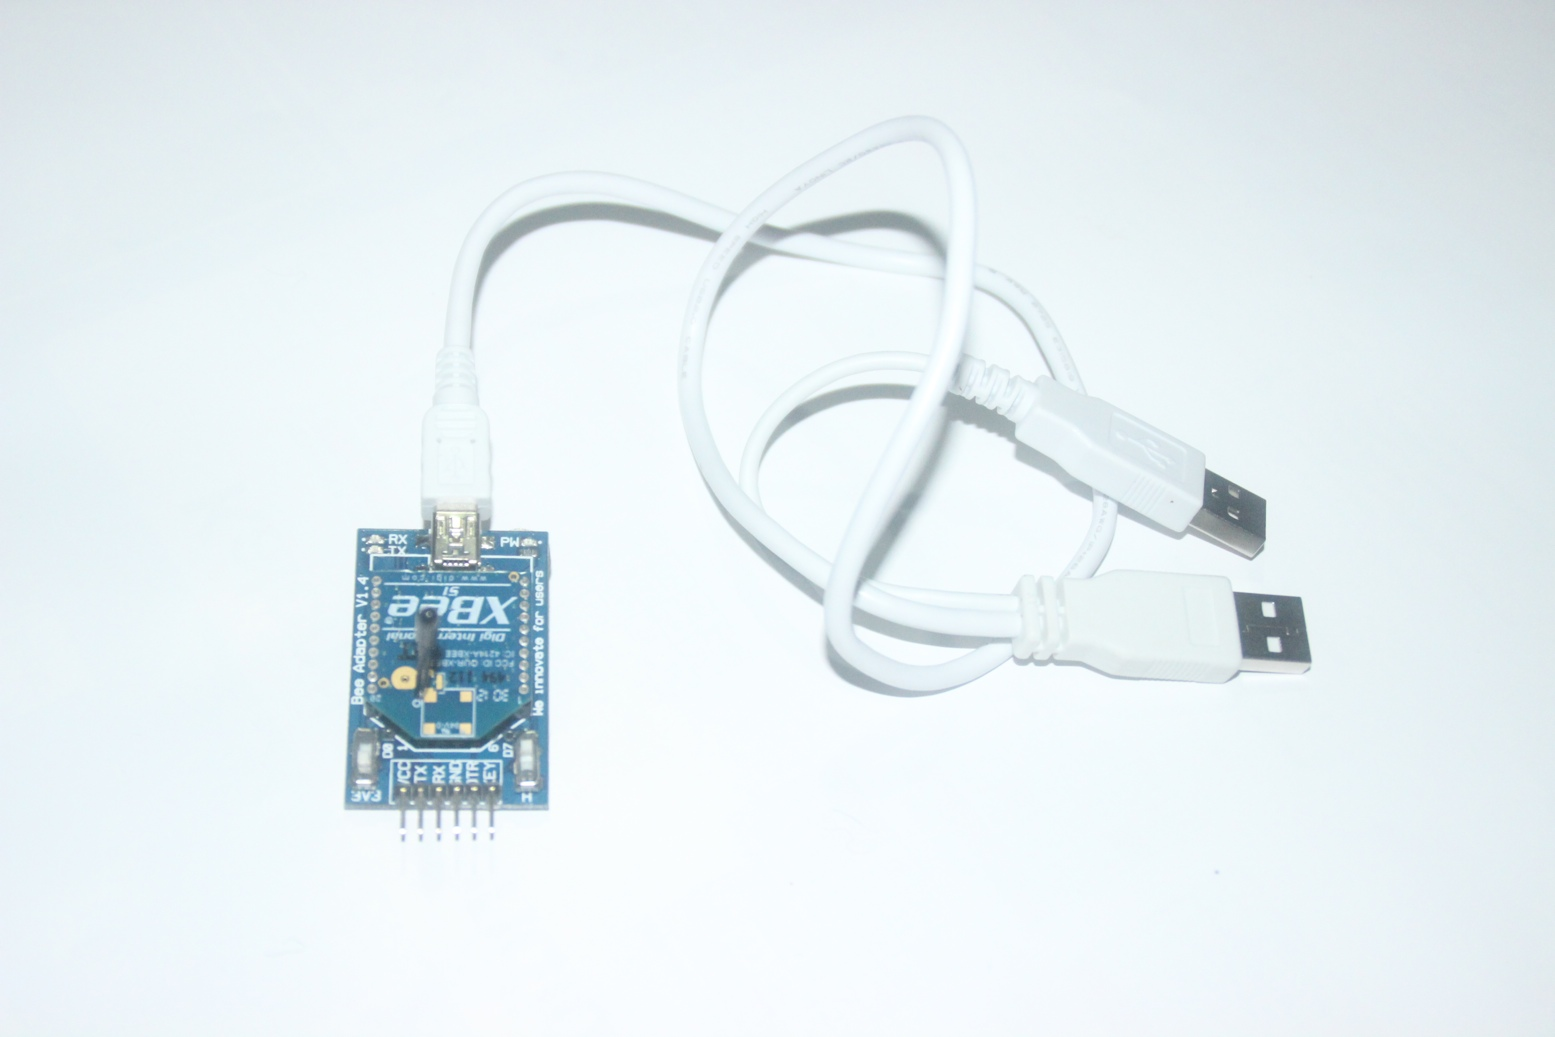
\includegraphics[width=0.7\textwidth]{gambar/xbee-sink-complete}
				    \caption{Koordinator XBee saat telah dirakit.}
				    \label{xbee-sink-complete}
				\end{subfigure}
				\caption{Koordinator peranti XBee yang akan disambungkan pada AP.}
				\label{xbee-sink}
			\end{figure}

			Merakit koordinator peranti XBee termasuk mudah, karena hanya perlu memasang \emph{XBee 802.15.4 Radios (Series 1)} pada \emph{XBee Explorer USB Board}, kemudian menghubungkan keduanya ke AP, seperti yang dapat dilihat pada Gambar \ref{xbee-sink-complete}.

			AP yang digunakan adalah TP-LINK MR3020 dengan USB Hub, seperti yang dapat dilihat pada Gambar \ref{ap-stripped}. USB Hub digunakan untuk menyambungkan USB \emph{flash drive}, koordinator IQRF, dan koordinator XBee.

			\begin{figure}[H]
				\begin{subfigure}[b]{\textwidth}
					\centering
				    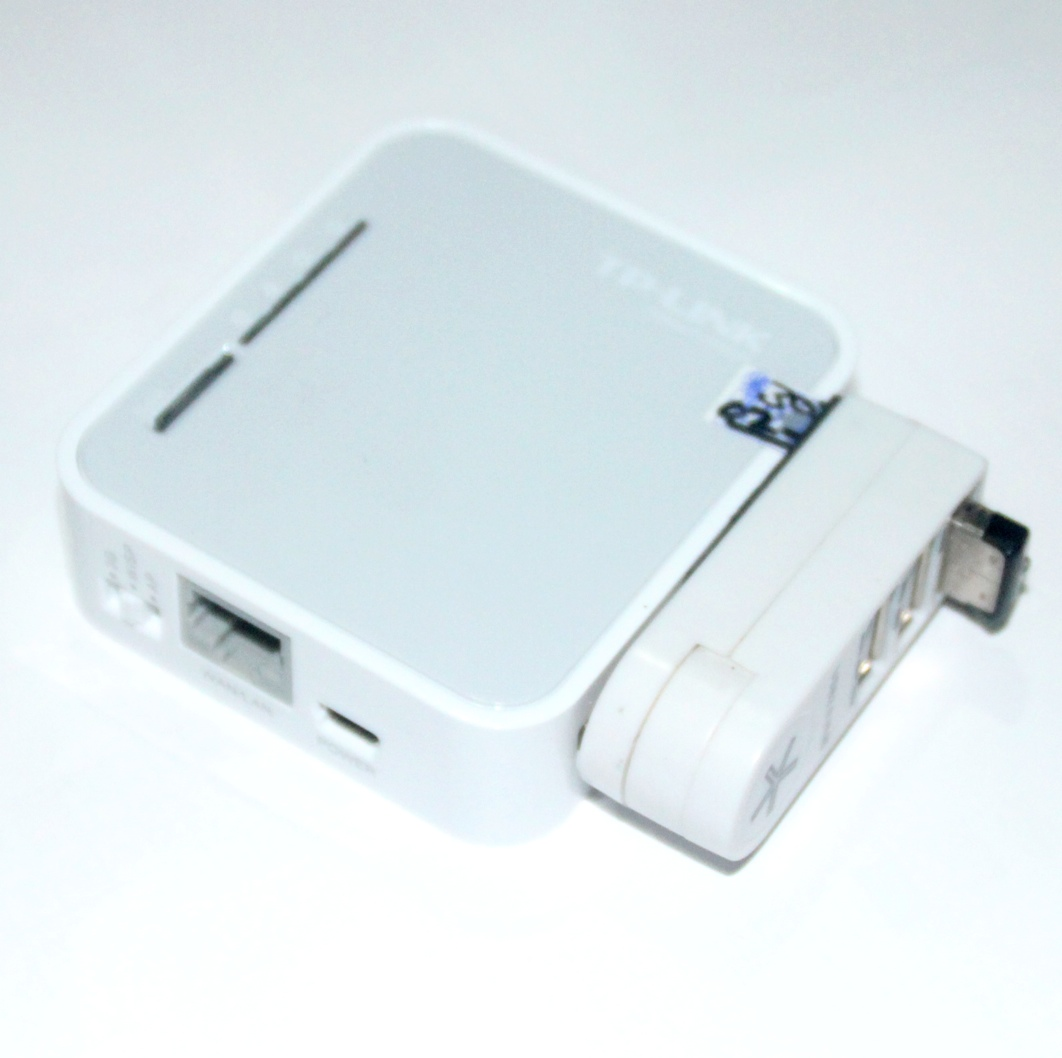
\includegraphics[width=0.5\textwidth]{gambar/ap-stripped}
				    \caption{AP saat sebelum dirakit.}
				    \label{ap-stripped}
				\end{subfigure}
				 ~
				\begin{subfigure}[b]{\textwidth}
					\centering
				    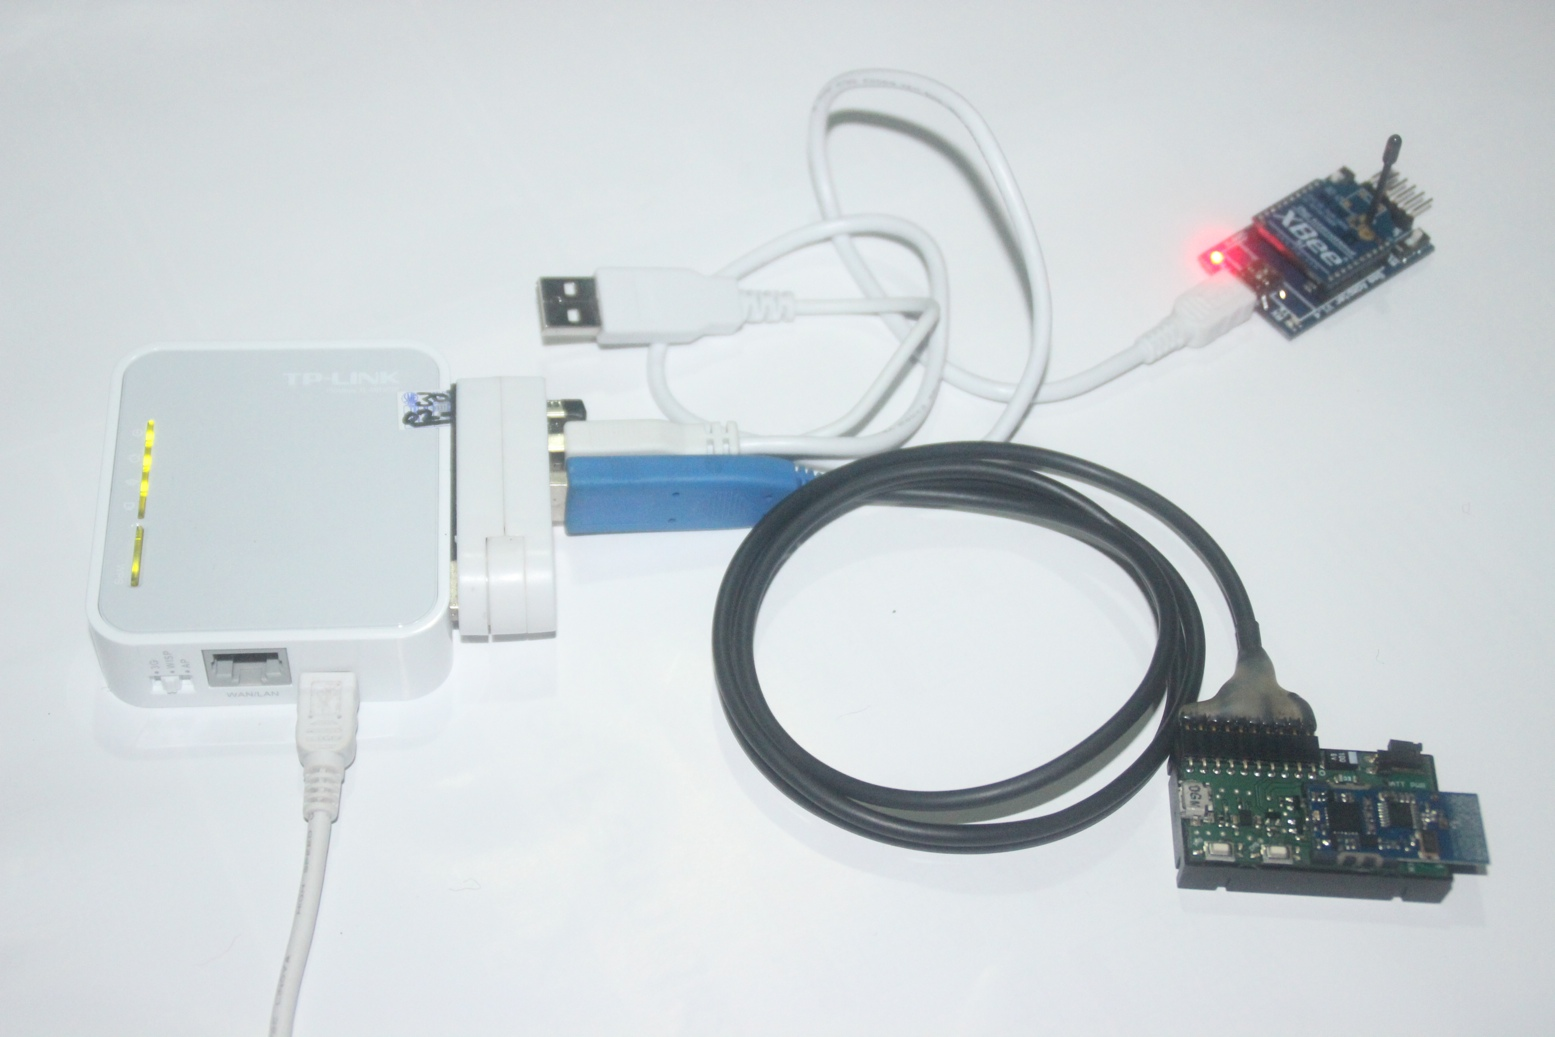
\includegraphics[width=0.7\textwidth]{gambar/ap-complete}
				    \caption{AP saat telah dirakit.}
				    \label{ap-complete}
				\end{subfigure}
				\caption{Koordinator peranti XBee yang akan disambungkan pada AP.}
				\label{xbee-sink}
			\end{figure}

			Urutan peranti yang terpasang ke AP, dari atas ke bawah, adalah USB \emph{flash drive}, koordinator XBee, dan koordinator IQRF. Posisi tersebut tidak boleh terbalik karena tidak sesuai dengan konfigurasi aplikasi yang sudah dirancang dan kembangkan. Sehingga kondisi saat semua peranti sudah dipasangkan dapat dilihat pada Gambar \ref{ap-complete}.

			Setelah AP sudah siap, langkah selanjutnya adalah perakitan sensor IQRF dan peranti XBee. Sensor-sensor IQRF terdiri atas TR-52B dan kit pengembangan DK-EVAL-03 seperti dapat dilihat pada Gambar \ref{iqrf-node}.

			\begin{figure}[H]
				\begin{subfigure}[b]{\textwidth}
					\centering
				    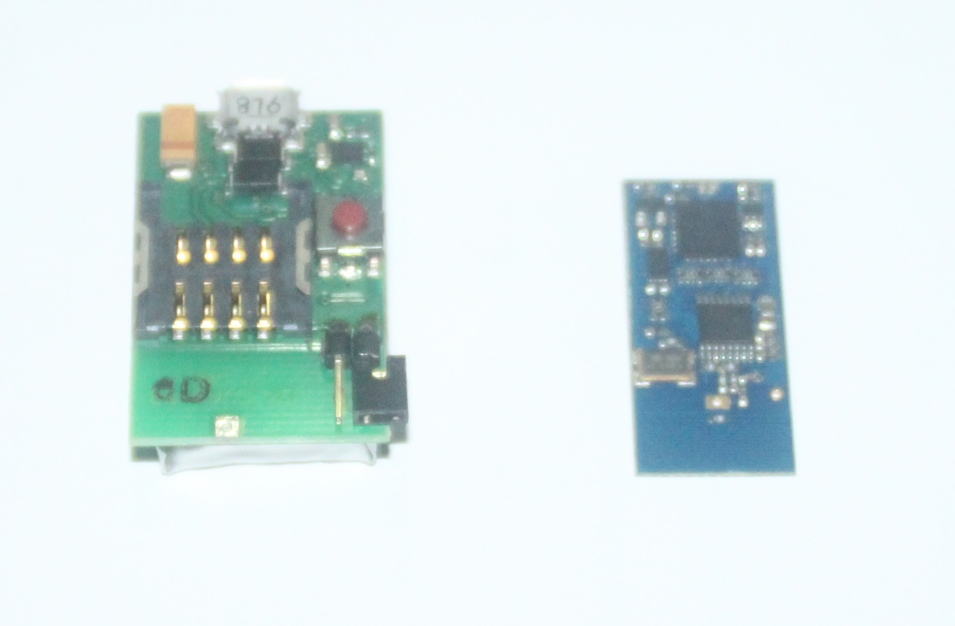
\includegraphics[width=0.4\textwidth]{gambar/iqrf-node-stripped}
				    \caption{Sebelum dirakit.}
				    \label{iqrf-node-stripped}
				\end{subfigure}
				 ~
				\begin{subfigure}[b]{\textwidth}
					\centering
				    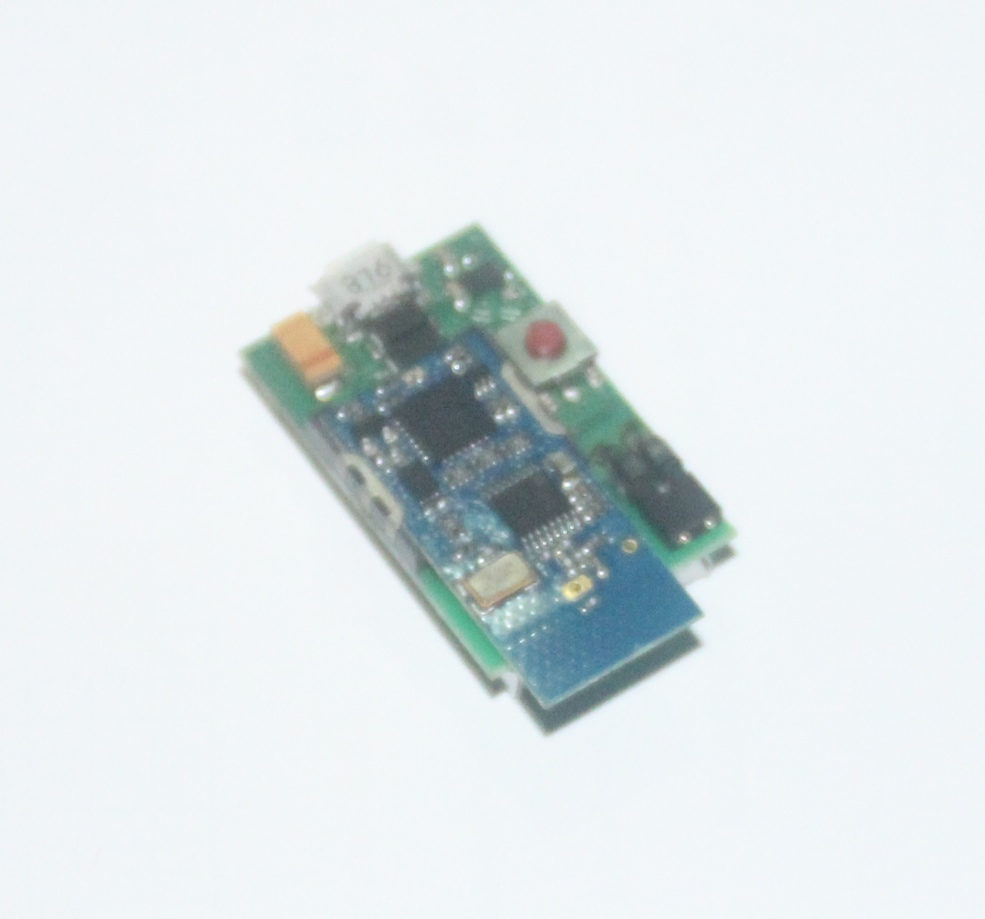
\includegraphics[width=0.4\textwidth]{gambar/iqrf-node-complete}
				    \caption{Setelah dirakit.}
				    \label{iqrf-node-complete}
				\end{subfigure}
				\caption{Sensor IQRF.}
				\label{iqrf-node}
			\end{figure}

			Untuk merakit sensor IQRF, masukkan TR-52B ke dalam kit pengembangan DK-EVAL-03 pada \emph{slot} yang sudah disediakan. Kondisi setelah dipasangkan dapat dilihat pada Gambar \ref{iqrf-node-complete}.

			Sedangkan peranti XBee relay terdiri atas tiga bagian, yaitu \emph{XBee 802.15.4 Radios (Series 1)}, \emph{2 channel Relay Shield For Arduino (With XBee/BTBee interface)}, dan Arduino Uno yang tersambung ke sumber listrik dengan kabel USB seperti dapat dilihat pada Gambar \ref{xbee-relay}.

			\begin{figure}[H]
				\begin{subfigure}[b]{\textwidth}
					\centering
				    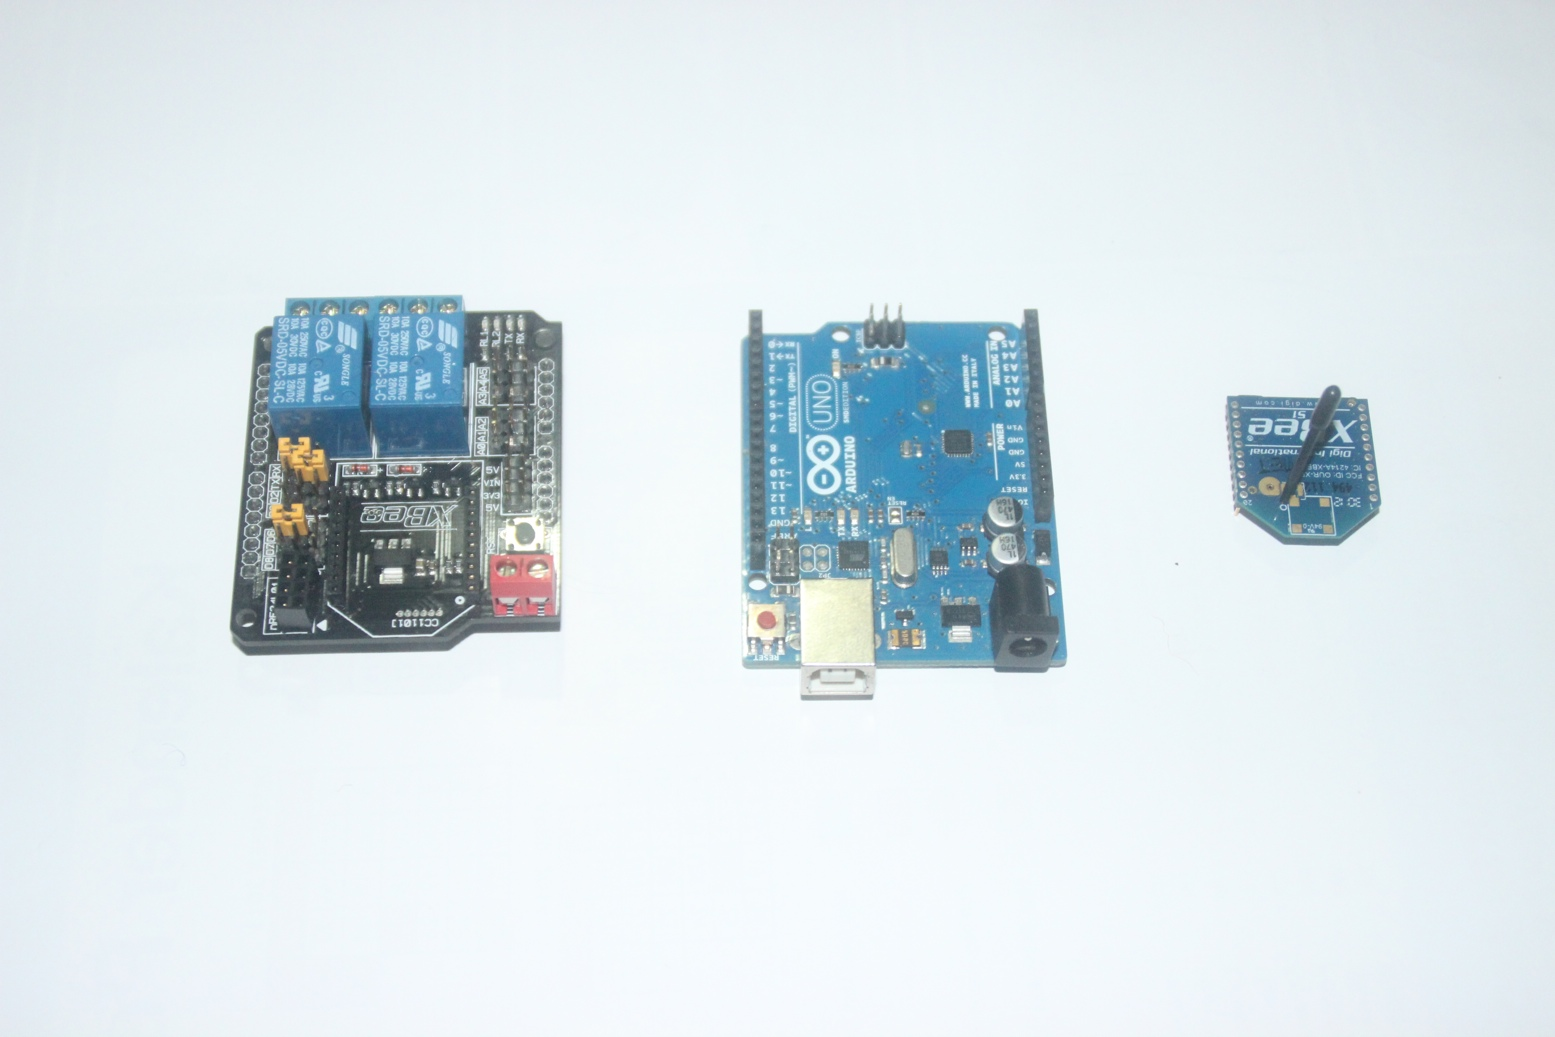
\includegraphics[width=0.7\textwidth]{gambar/xbee-stripped}
				    \caption{Sebelum dirakit.}
				    \label{xbee-stripped}
				\end{subfigure}
				 ~
				\begin{subfigure}[b]{\textwidth}
					\centering
				    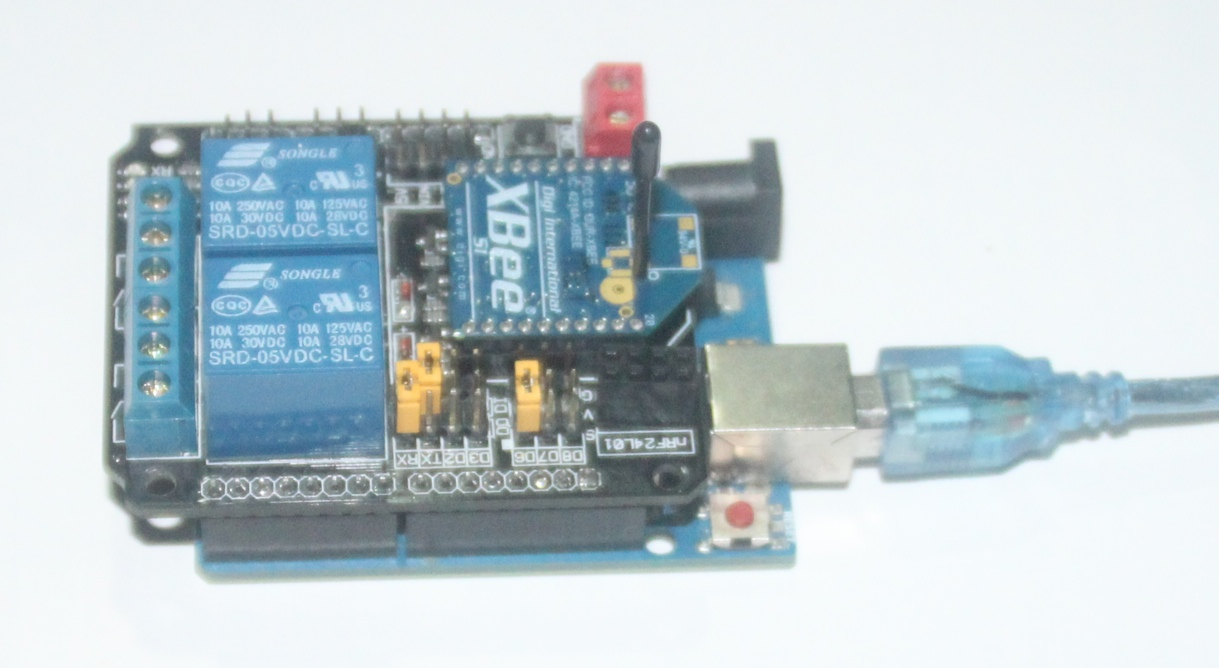
\includegraphics[width=0.7\textwidth]{gambar/xbee-complete}
				    \caption{Setelah dirakit.}
				    \label{xbee-complete}
				\end{subfigure}
				\caption{Peranti XBee.}
				\label{xbee-relay}
			\end{figure}

			Peranti XBee akan tersusun dalam tiga lapis rangkaian, mulai dari bawah, Arduino Uno, \emph{2 channel Relay Shield For Arduino (With XBee/BTBee interface)}, dan \emph{XBee 802.15.4 Radios (Series 1)}. Hasil rakitan peranti XBee dapat dilihat pada Gambar \ref{xbee-complete}.

		\subsection{Hasil Uji Coba Aplikasi}
			Uji coba yang dilakukan menggunakan satu set AP lengkap yang sudah dilengkapi dengan koordinator IQRF dan XBee. Sensor yang digunakan adalah dua buah IQRF dan satu buah XBee.

			Uji coba pertama dilakukan dengan penambahan XBee Relay baru via aplikasi web dan menyalakan relay 1 dengan ponsel cerdas seperti dapat dilihat pada Gambar \ref{xbee-action}. Pada Gambar \ref{xbee-action} dapat dilihat bahwa relay 1 dalam keadaan menyala pada layar ponsel cerdas dan XBee Relay.

			\begin{figure}[H]
			  \centering
			    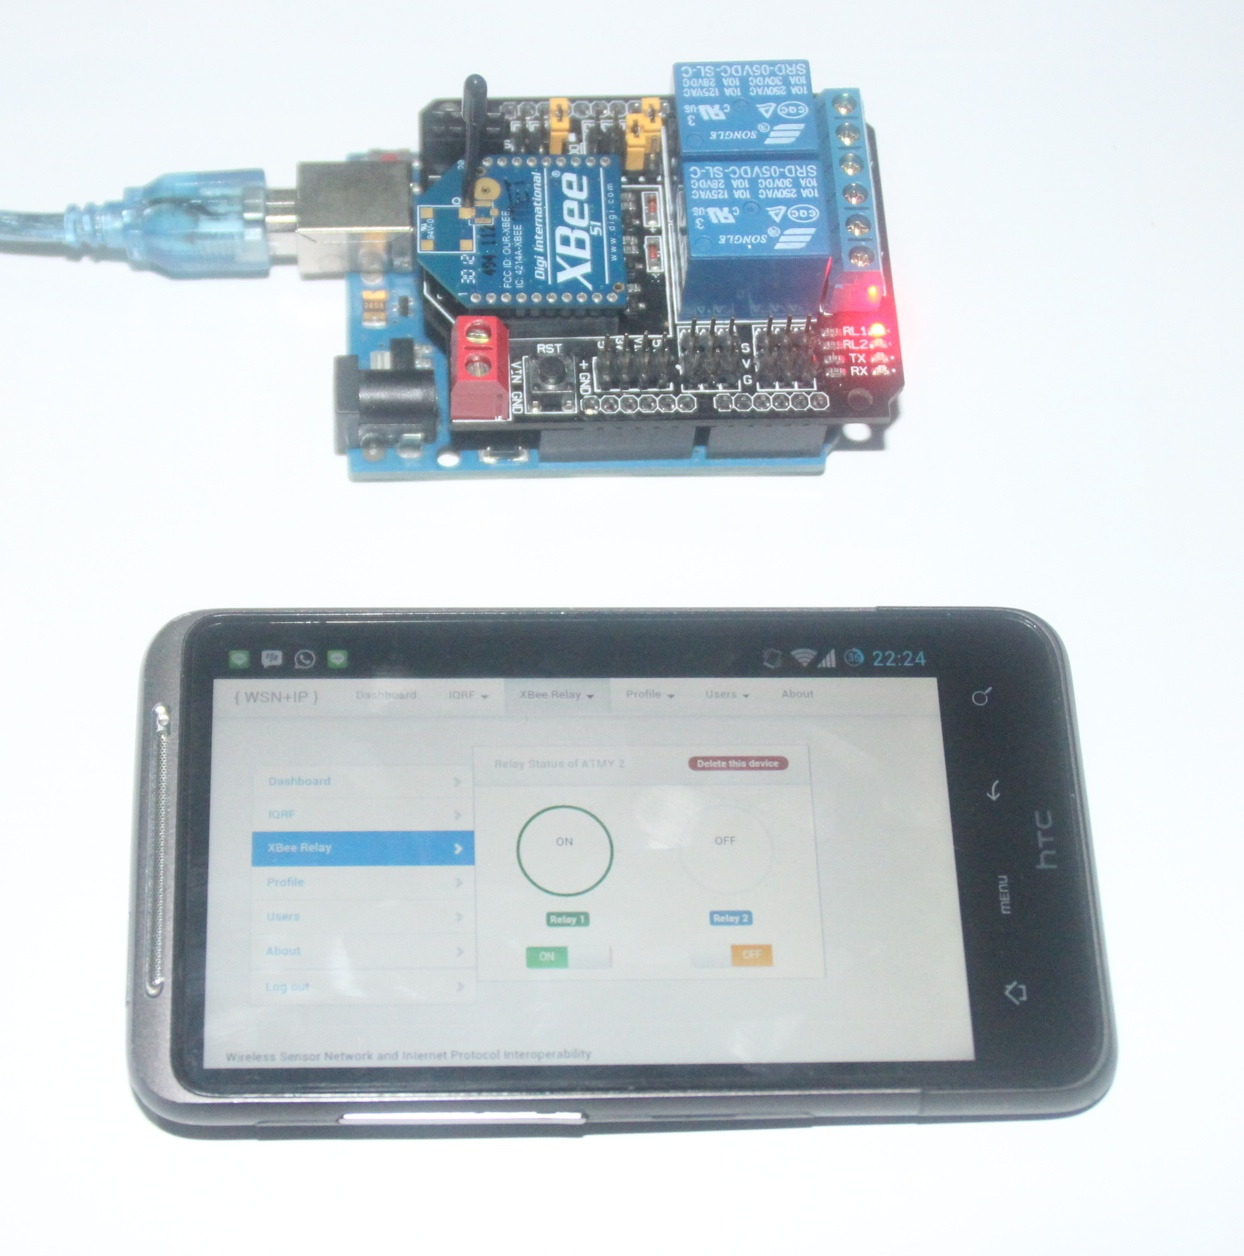
\includegraphics[width=0.7\textwidth]{gambar/xbee-action}
			    \caption{Uji coba aplikasi dengan ponsel cerdas.}
			    \label{xbee-action}
			\end{figure}

			Pada saat pengguna meng-klik salah satu saklar, akan tampak \emph{progress} dari proses menyalakan relay berupa garis tapi lingkaran berwarna hijau. Saat relay sudah dalam kondisi menyala, maka lingkaran akan mempunyai garis tepi berwarja hijau yang sempurna.

			Pengujian IQRF dilakukan dengan penambahan dua sensor via aplikasi web dan kemudian melihat temperatur yang terbaca. Salah satu sensor digenggam dengan tangan untuk memanipulasi temperatur. Hasilnya dapat dilihat pada Gambar \ref{screenshot-iqrf}.
			
			\begin{figure}[H]
			  \centering
			    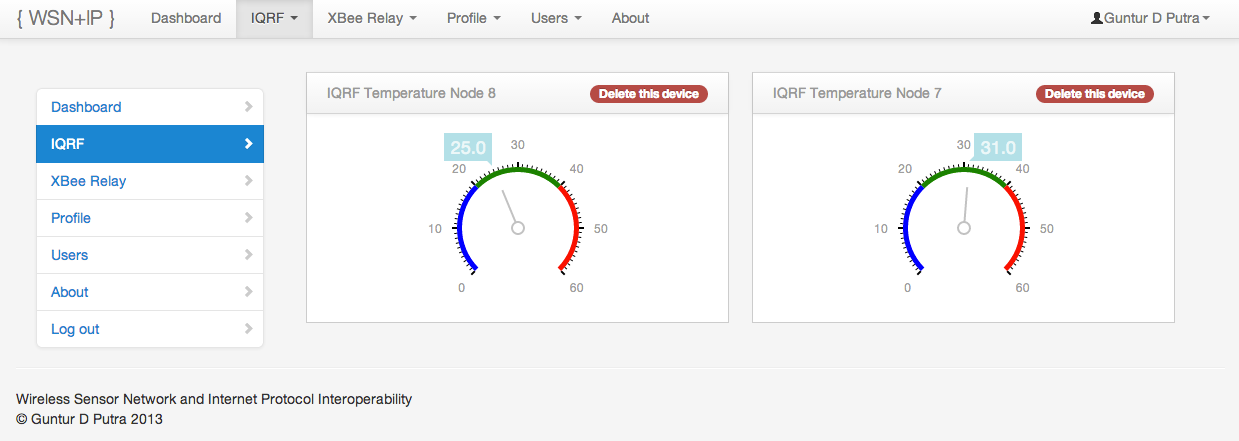
\includegraphics[width=0.9\textwidth]{gambar/screenshot-iqrf}
			    \caption{Membaca temperatur yang terbaca pada sensor.}
			    \label{screenshot-iqrf}
			\end{figure}

			Jarum penunjuk pada masing-masing penampil akan bergerak sesuai dengan bacaan temperatur dari masing-masing sensor IQRF. Gerakan akan terjadi secara langsung, tanpa pengguna harus memuat ulang halaman web.
			
			Dari hasil pengujian di atas, didapati bahwa aplikasi yang dibangun sudah dapat berfungsi sebagaimana mestinya.

		\subsection{Masalah dan Penyelesaian}
			Masalah yang pertamakali muncul adalah tentang extroot. TP-LINK MR3020 memiliki \emph{bug} yang membuat memori eksternal tidak berfungsi saat \emph{booting} pertamakali. Setelah TP-LINK MR3020 dijalankan ulang, memori eksternal baru terbaca. Penyebab dari masalah ini belum ditemukan, sehingga solusi untuk masalah ini adalah melakukan \emph{rebooting} jika TP-LINK MR3020 tidak membaca memori eksternal. Masalah ini tidak ditemukan pada AP dengan jenis lain.

		%	Komunikasi serial yang kata perkata.
			
			IQRF dinilai kurang stabil, terlebih saat menancapkan kabel USB to Serial Prolific ke USB Hub pada AP saat AP sudah menyala. Jika kurang berhati-hati, AP justru akan menjadi tidak stabil. Gejala yang muncul seperti pustaka PHP yang tidak terbaca, sampai jaringan Wi-Fi yang terputus. Untuk mengantisipasi masalah ini, sebaiknya semua kabel terpasang sebelum AP dinyalakan.
			
% Baris ini digunakan untuk membantu dalam melakukan sitasi.
% Karena diapit dengan comment, maka baris ini akan diabaikan
% oleh compiler LaTeX.
\begin{comment}
\bibliography{daftar-pustaka}
\end{comment}

%-------------------------------------------------------------------------------
%                            	BAB V
%               		KESIMPULAN DAN SARAN
%-------------------------------------------------------------------------------

\chapter{KESIMPULAN DAN SARAN}

\section{Kesimpulan}
	Berdasarkan hasil analisis dan pengujian fungsional aplikasi ini, didapat kesimpulan sebagai berikut:

	\begin{enumerate}
		\item Interoperabilitas \emph{Wireless Sensor Network} (WSN) \emph{multiple vendor} dengan \emph{Internet Protocol} (IP) dapat tercapai dengan \emph{gateway} yang ditanamkan aplikasi berbasis web yang didukung dengan aplikasi Python untuk berkomunikasi dengan WSN yang terisi dengan aplikasi C.

		\item Sesuai pengujian yang dilakukan dalam skala laboratorium, aplikasi dapat berjalan baik sesuai dengan fitur-fitur yang dirancang.

		\item Salah satu kendala yang dihadapi adalah tidak stabilnya AP seri TP-LINK MR3020 dalam pembacaan memori eksternal. Saat pertama kali dinyalakan, AP tidak membaca memori eksternal yang sudah dipasang. Setelah AP dinyalakan ulang, baru AP dapat membaca memori eksternal.

		\item Masalah lain yang dihadapi juga masalah ketidakstabilan koordinator IQRF yang tertancap pada AP. Agar tidak terjadi kesalahan perangkat keras, sebaiknya koordinator IQRF sudah terpasang pada saat AP masih dalam kondisi mati.
	\end{enumerate}


\section{Saran}
	\begin{enumerate}
		\item Penelitian selanjutnya dapat menggunakan AP selain TP-LINK MR3020 sebagai gateway dan membandingkannya dengan performa TP-LINK MR3020 yang memiliki \emph{bug} pada extroot.
		\item Penelitian ini menggunakan Python untuk berkomunikasi dengan kanal serial, penelitian selanjutnya dapat menggunakan pendekatan yang lain, seperti membangun aplikasi dengan bahasa C.
		\item Penelitian selanjutnya dapat menggunakan jenis-jenis WSN yang lebih bervariatif guna interoperabilitas yang lebih luas.
	\end{enumerate}

	
% Baris ini digunakan untuk membantu dalam melakukan sitasi
% Karena diapit dengan comment, maka baris ini akan diabaikan
% oleh compiler LaTeX.
\begin{comment}
\bibliography{daftar-pustaka}
\end{comment}


%-----------------------------------------------------------------
%Disini akhir masukan Bab
%-----------------------------------------------------------------

%-----------------------------------------------------------------
%Disini awal masukan untuk Daftar Pustaka
%-----------------------------------------------------------------
%%\nocite{Abel2010,Guerbas201350}
%%\bibliography{research-plan}
%%\bibliographystyle{plainnat}
\begin{thebibliography}{9}

\bibitem[satu(2013)]{satu01}
Spinar, R., dkk, ``Demo Abstract: Efficient Building Management with IP- based Wireless Sensor Network'', , 6th European Conference on Wireless Sensor Networks. Cork, Ireland 11-13 February 2009.

\bibitem[dua(2013)]{dua02}
Adam Dunkels, Thiemo Voigt, Niclas Bergman, dan Mats Jonsson ``The Design and Implementation of an IP-based Sensor Network for Intrusion Monitoring'', Swedish National Computer Networking Workshop, Sweden, 2004.

\bibitem[tiga(2013)]{tiga03}
Sigit B. Wibowo, dan Widyawan, ``Wireless Sensor Network and Internet Protocol Integration with COTS'', 2013 AUN/SEED-Net Regional Conference in Electrical and Electronics Engineering, Bangkok, Thailand, 2013.

\bibitem[empat(2013)]{empat04}
Dokumen online, http://www.iqrf.org/, IQRF, diakses pada Maret 2013

\bibitem[lima(2013)]{lima05}
Widyawan, Sigit B. Wibowo, dkk, ``iHome: Low-Cost Domotic for Residential Houses'', 5th AUN/SEED-Net Regional Conference on Information and Communications Technology (RCICT), Manila, Filipina, 2012.

\bibitem[enam(2013)]{enam06}
Dokumen online,https://openwrt.org/, diakses pada Maret 2013

\bibitem[tujuh(2013)]{tujuh07}
Dokumen online, http://www.digi.com/technology/rf-articles/wireless-zigbe,
diakses pada Maret 2013.

\end{thebibliography}
\addcontentsline{toc}{chapter}{DAFTAR PUSTAKA}
%-----------------------------------------------------------------
%Disini akhir masukan Daftar Pustaka
%-----------------------------------------------------------------

\end{document}